%% FELthesis: LaTeX class for bachelor, master, and phd thesis in CTU FEL
%% template.tex: template file
%% (c) 2012 Vít Zýka, vit.zyka@seznam.cz
%%
%% 2012-12-17 v0.1 first version derived from cmpthesis.tex

\documentclass[msc,draft,czech]{felthesis} % or [...,czech] for thesis in Czech
%%\documentclass[msc,draft]{felthesis} % or [...,czech] for thesis in Czech
%%\documentclass[phd,draft]{felthesis} % or [...,czech] for thesis in Czech

%% --- your additional packages:
\usepackage[utf8]{inputenc}
\usepackage{algorithm}
\usepackage{algorithmicx}
\usepackage{algpseudocode}
\usepackage{setspace}

%% --- usefull draft packages
%%\usepackage[notref]{showkeys} % show labels for referencies
%%\usepackage{showlabels}       % similar
%%\usepackage{showidx}          % show index entries on every page

%% ======================================================== thesis info
\startThesisInfo
  \Title{Dynamické vyvažování obtížnosti her pomocí metod teorie her}
  \Author{Lukáš Beran}
  \AuthorEmail{beranlukas@gmail.com} % optional
  %\ThesisUrl{http://fel.cvut.cz/???/???-bsc.pdf} % optional
  \Date{Květen 2013}
  \Department{Katedra kybernetiky}
  \Advisor{Branislav Bošanský}
  \KeywordsCz{Dynamické vyvažování obtížnosti her; adaptivní UI; teorie her; \dots}
  \KeywordsEn{Dynamic difficulty game balancing; adaptive AI; game theory; \dots}
  %\AssignmentPage{assignment.pdf} % insert official assignment if given
\stopThesisInfo

%% ============================== your definitions (abbreviations etc.)
%%\def\Ax{\mathbf{A}_{x}}

%% =========================================================== settings
\graphicspath{{fig/}{logo/}} % subdirectories where TeX finds pictures
%\bibliography{beranlu6mst.bbl}
\addbibresource{beranlu6mst.bib} % bibliography file
\onehalfspacing
%%\renewcommand{\baselinestretch}{1.5}

%% ========================================================== text body
\begin{document}

\MakeTitle

\startFrontMatter
  \startAcknowledgement
Text of acknowledgement\dots
\stopAcknowledgement

\endinput
%%
%% End of file `acknowledgement.tex'.

  \startDeclaration
\ifCzech
  Prohlašuji, že jsem předloženou práci vypracoval samostatně,
  a~že jsem uvedl veškeré použité informační zdroje v~souladu
  s~Metodickým pokynem o~dodržování etických principů při přípravě
  vysokoškolských závěrečných prací.
\fi
\ifEnglish
  I declare that I worked out the presented thesis independently
  and I quoted all used sources of information in accord with
  Methodical instructions about ethical principles for writing
  academic thesis.
\fi
\stopDeclaration

\endinput
%%
%% End of file `declaration.tex'.

  \startAbstractCz
  Text abstraktu česky\dots
\stopAbstractCz

\startAbstractEn
  Text of abstract in English\dots
\stopAbstractEn

\endinput
%%
%% End of file `abstract.tex'.

  \tableofcontents
  \setcounter{secnumdepth}{2}
	\listoffigures
  \startAbbreviations{%
  Preliminary text\dots
}
\abbrv[abbrv.]  explanation
\abbrv[...]     ...
\stopAbbreviations

\endinput
%%
%% End of file `abbreviations.tex'.

\stopFrontMatter

\floatname{algorithm}{Algoritmus}

\startBodyMatter
  %\includeonly{ch01}
  \chapter{Úvod}
Some introductory text\dots

\section{Definice}

Dynamické vyvažování obtížnosti (dynamic difficulty adjustement, DDA) je obecným konceptem, jak přistupovat k návrhu programů, jež jsou využívány uživateli rozdílných schopností a zkušeností. 

Klasickým přístup je předdefinování několika rozdílných nastavení s odlišnými požadavky na dovednosti uživatelů, kteří si mezi těmito nastaveními volí ručně. Naopak dynamický, adaptivní přístup volbu nastavení nechává alespoň z části na samotném programu, který se rozhoduje na základě modelu uživatele.

Se zkratkou DDA se nejčastěji setkáme v oblasti počítačových her a simulací, ale toto prostředí není závaznou podmínkou. Příklady budou uvedeny v sekci \ref{sec:aplikacedda}. Cílem DDA je přizpůsobovat proměnné systému co nejlépe aktuálním potřebám uživatele.  S typem aplikace úsce souvisí druh potřeb uživatele. Lišit se budou potřeby pacientů využívajících rehabilitační programy a potřeby hráčů počítačových her. Dále se v textu zaměřím na využití DDA v počítačových hrách, případně v tzv. serious game, které mají za úkol udržet uživatele u užitečné činnosti formou zábavné hry.

Synonymy pro DDA jsou např. dynamic difficulty balancing, dynamic game balancing, auto-dynamic difficulty, adaptive difficulty. Ve čtyřech z pěti pojmů se vyskutuje slovo difficulty (obtížnost), které jsem doposud nezmínil. Vyvažování obtížnosti je základem velké většiny hry využívající koncept DDA. Myšlenka za tím je jednoduchá. Je-li hra pro hráče příliš snadná, hráč se nudí, hru opustí. Naopak je-li hra příliš obtížná, hráč je frustrován, hru opouští. V obou případech hra ztrácí své uživatele. U komerčních produktů se pak jedná o ztrátu financí. U programu využívaném při rehabilitaci se pak jedná o ztrátu motivace v pokračovaní rehabilitací. Obtížnost hry tedy přímo souvisí s její zábavností a udělat hru zábavnou pro co největší masu lidí je cílem DDA. Míra zábavnosti hry není závislá pouze na její obtížnosti. Jak lze definovat zábavu a jak ji lze měřit více popíši v kapitole \ref{sec:defzab}. 

Každé využití auto-dynamického vyvažování hry lze zařadit do několika kategorií z různých úhlů pohledu. Různé hry vyžadují různé přístupy a je dobré se zamyslet nad konkrétní hrou. Vybrat si z jakých kategorií by mělo být DDA použito. Designér hry by si měl položit několik následujících otázek :

\begin{enumerate}
	\item Měl by hráč vědět, jestli je DDA použito?
	\item Má být obtížnost měněna v průběhu hry, nebo pouze na začátku?
	\item Je hlavním cílem hry zábava, nebo něco jiného?
	\item Jakým způsobem může být ovlivňována obtížnost hry?
\end{enumerate}

Dle svých odpovědí každý určitě zvládne zařadit hru do následujících kategorií.

\subsection{Explicitní a implicitní}

První dělení rozlišuje stav, kdy je hráč obeznámen s dynamickou obtížností a kdy naopak je mu to zatajeno. Jestliže hráč dopředu ví, že se obtížnost hry mění dle jeho konání, jedná se o explicitní DDA. Pokud je snaha utajit dynamickou změnu obtížnosti, jedná se o implicitní DDA.

Explicitní použití by mělo být dobře známé i ze všedního života. Když mezi s sebou v něčem soutěží týmy, kteří nejsou svými schopnostmi vyrovnaní, často se přistoupí k nějakému handicapu pro ty silnější. Ať už se jedná o věnování náskoku při závodu v běhu mladšímu z bratrů, či o posazení zdravého člověka do kolečkového křesla na paralympiádě. 

Příkladem ze světa deskových her může být ve hře Go povolení slabšímu hráči na začátku hry zahrát několik svých kamenů navíc, nebo naopak odebrání některých figur ve hře šachy hráči silnějšímu.

Někdy zařazení hry nemusí být zcela jednoznačné. Mnoho hráčů z laické veřejnosti je si vědomo podvádění v závodních hrách jako je Mario Kart, či Need For Speed, přestože se o tom nedozvědí v pravidlech hry. V případě, že se vývojáři rozhodnou pro implicitní DDA, měli by jej navrhnout tak, aby jej hráč neodhalil. Jestliže o něm každý ví, asi už není zcela korektní hru zařadit do implicitní kategorie.

\begin{figure}
  \centering
  
\includegraphics[width=0.5\textwidth]{ch1mariokart2}
	\caption{Ukázka špatného vyvažování hry u hry Mario Kart dává prostor pro vytváření vtipů. \cite{15UnTrue} }
	\label{ch1mariokart2}
\end{figure}

Nejasná kategorizace může být i v opačném případě. Mějme jako příklad moderní deskovou hru Vysoké napětí. Ve hře existují pravidla závislá na aktuálním pořadí hráčů a snaží se pomáhat prohrávajícím hráčům a naopak ubližovat těm ve vedení. U Vysokého napětí hráči nakupují suroviny v opačném pořadí než si vedou. Stejné suroviny mají rozdílnou cenu. Poslední hráč vykoupí nejlevnější suroviny a naopak na toho prvního zůstanou ty nejdražší. Za stejnou věc zaplatí různě, a tedy se zvýší šance posledního hráče dostat se do vedení. Přestože toto pravidlo je všem zúčastněným známo, tak asi málokdo o něm přemýšlí jako o dynamické vyvažování obtížnosti hry.

\subsection{Dynamická a statická}

Obtížnost hry lze přizpůsobovat před začátkem hry nebo v jejím průběhu. Dle toho se rozděluje DDA na statickou(offline), či dynamickou(online). Typický příkladem offline adaptivity bude zpracování hráčových dat a úprava hry během jejího načítání. Z tohoto důvodu je offline adaptivita zaměřena především na generování herního světa, herních scénářů a úkolů\cite{16Survey}. Příkladem mohou být hry Fallout 3 a Fallout: New Vegas, kde se při vstupu na nové území generují nepřátelé, a to dle levelu hráčova avatara. Offline adaptivitu lze považovat za jedinou možnou při vytváření různých logických hádanek a her. Na základě rychlosti řešení/nedokončení předchozí hádanky, lze vygenerovat hádanku novou lépe odpovídající hráčovým schopnostem. Tímto problémem se zabývá článek Automatic Generation of Game Elements via Evolution\cite{17Evol}, kde testovanými hrami byla hra se šachovými figurami a hra procházení barevným bludištěm.

Online adaptivita bude naopak zaměřena na adaptivitu umělé inteligence NPC a úpravu pravidel hry. Vede-li si hráč příliš dobře v závodní hře, ostatním hráčů se zvýší maximální rychlost. Ztratí-li hráč příliš životů, v rohu v další místnosti se objeví lékárnička. Adaptivita může být samozřejmě i druhým směrem. Sebere-li hráč soupeři důležité figurky v deskové hře šachy, soupeři se zvýší "inteligence", začne uvažovat na více kol dopředu. 

Online adaptivitu můžeme zasadit přímo do principů hry. Ve hře Pocket Billiards hrají proti sobě dva hráči na kulečníkovém stole. Na stole je několik koulí dvou barev. Každý hráč má přiřazenou jednu z barev a jeho úkolem je dostrkat své koule do děr dříve než to udělá soupeř. Adaptivita je zde dána samotným principem hry. Dostane-li se jeden hráč do vedení a odstraní z plochy znatelně více koulí než jeho soupeř, pak je pro něj stále obtížnější dostat další koule do děr. Zároveň se zvyšuje pravděpodobnost, že bude muset provést takový šťouch, který může odstranit z plochy soupeřovu koule, a tedy mu tím může pomoci dorovnat skóre.\cite{5}

\section{Aplikace DDA} \label{sec:aplikacedda}

Algoritmy vyvažování obtížnosti lze využít v širokém spektru aplikací. Mohou být vhodné všude tam, kde je vyžadována určitá dovednost, schopnost. V takovém případě může být obtížné aplikaci, program navrhnout tak, aby byl dobře využitelný velkým spektrem lidí různých schopností.

DDA můžeme nalézt nejen v zábavním průmyslu, ale i u vážných her. Adaptivní obtížnost programu může zefektivňovat léčbu nemocných lidí, nahrazovat osobního trenéra či učitele. V následujících 4 podkapitolách popisuji konkrétní užití dynamické obtížnosti v komerční i v akademické sféře.

\subsection{Zábavní průmysl}

Hráče počítačových her lze rozdělit dle jejich schopností od příležitostných až po hardcore hráče. Většina her obsahuje statickou volbu obtížnosti na začátku hry. V některých případech to nemusí být dostačující, a proto se tvůrci komerčních her snaží více, či méně úspěšně implementovat adaptivní obtížnost.

Na stránce \cite{1} lze nalézt desítky příkladů všech různých žánrů. Do následujícího seznamu 5 her jsem vybral ty známější příklady.


\subsubsection{Left 4 Dead}
\label{sec:Left4Dead}

V zombie hře Left 4 Dead pojmenovali adaptivní systém The AI Director. Na základě aktuálního hráčova zdraví, munice a relativní pozice v rámci dané úrovně hry The AI Director generuje ve hře zbraně, munici, lékárničky na pomoc hráči a naopak generuje lehčí, či těžší nepřátele. Např. blíží-li se hráč konci úrovně a má plné zdraví i munici, hra vygeneruje těžkého soupeře „Tank“. \cite{2}

\subsubsection{Max Payne 3}

Hra Max Payne 3 obsahuje celkem 5 statických obtížností(Easy, Medium, Hard, Hardcore, Old School), které se v průběhu hry adaptivně přizpůsobují hráči. Čím nižší obtížnost si hráč na začátku zvolí, tím více se hra může měnit ve prospěch hráče.

Jestliže hráč opakovaně umírá, dostane se mu pomoci ve formě bonusových léků(painkillers), které umožní lehčí projití daného úseku hry. Při smrti na lehkou a střední obtížnost se hráčův avatar obnoví minimálně s jedním plným zásobníkem pro každou zbraň vyjma granátometů. Plus za každé tři úmrtí ve stejném úseku dostane jeden painkiller navíc až do maximálního limitu devíti painkillerů.
Na těžkou obtížnost je dynamická obtížnost více limitovaná. Jestliže hráč zemře 5 krát po sobě, dostane jeden painkiller. Pokud zemře podesáté, dostane druhý painkiller. Další léky mu hra již nepřidává. \cite{3}

\subsubsection{The Elder Scrolls IV: Oblivion}

Dalším příkladem mohou být hry Oblivion a Fallout 3 od Bethesda Softworks. V Oblivionu nepřátelé levelují s hráčem. Stráže ve městě mají level o 2-5 vyšší než vy, banditi mají level o 2-5 nižší atd. Tímto je docíleno, že se můžete vydat kamkoli ve hře aniž byste narazili na příliš obtížné nepřátele. Mimo síly nepřátel se adaptivně upravuje druh nepřátel, jejich vybavení, nabízení zboží v obchodech apod. Občas může docházet k nelogickým situacím, kdy obyčejní potulní bandité mají na sobě nejmodernější brnění, nebo kdy máte za úkol donést vlčí kožešinu ve světe, kde už tak slabí nepřátelé se nepohybují. \cite{4}

\subsubsection{Mario Kart Wii}

Závodní simulátory jsou dobře známé využíváním adaptivní obtížnosti her a mezi nejznámější zástupce patří arkádové závody Mario Kart. Ve hře se adaptivně mění rychlost protivníků a také bonusové power-upy, které můžete sbírat. Hra podporuje natolik prohrávající hráče, že ať už je aktuální stav hry jakýkoli, může vyhrát kdokoliv.

Což lze brát jako velkou výhodu, kdy žádný z hráčů nemá důvod ke vzdávání hry. Nevýhodou je právě známost a odhalení tohoto systému, a tudíž je lehce zneužitelná. Např. konkrétně ve variantě Mario Kart Wii je vedoucí hráč na začátku posledního kola bombardován modrým krunýřem, či jinou devastující zbraní a je záhy poslán na poslední místo. Nejlepší strategií je projet do posledního kola na druhé pozici, což moc nedává smysl. \cite{5}

\subsubsection{Pro Evolution Soccer 2008}

Úspěšný fotbalový simulátor Pro Evolution Soccer se ve své verzi s číslem 2008 chlubil adaptivním systémem nazvaný Teamvision. Teamvision se učí od hráče jeho styl hry a snaží se upravovat taktiku svého týmu, aby co nejlépe reagovala na tu soupeřovu. Použití jedné finty může fungovat jednou, dvakrát, ale později již naprosto stejná finta nevede k vítězství. \cite{6}

\subsection{Cvičení}

Herní zařízení jako jsou Microsoft Kinect a Nintendo Wii dávají prostor pohybovým hrám. Stejně jako v jiných příkladech i zde platí, že existují lidé s diametrálně odlišnou fyzickou kondicí. Kondice se v ideálním případě při opakované hře stále zlepšuje, a proto je vhodné k tomu přizpůsobovat obtížnost hry.

Příkladem takové aplikace může být jednoduchá chodící hra hratelná v internetovém prohlížeči, jež má za úkol motivovat starší lidi k pohybu.

V druhém případě nebylo využito žádné ze zmíněných zařízení. Autoři článku \cite{7} se zaměřili na jogging v páru. 

\subsubsection{Podpora pohybu starších lidí}

Evropská populace stárne a odmítání pohybu staršími lidmi se stává závažným problémem. Z nedostatku fyzické námahy klesá síla a ohebnost těchto lidí, ztrácejí kostní hmotu a tím zvyšují pravděpodobnost pádu a zlomení některé z končetin. Z tohoto důvodu se skupina z Technologického institutu zaměřila na vývoj hry, jež má starší lidi motivovat k pohybu a jejíž nedílnou součástí je vyvažování obtížnosti. \cite{8}

Hra je vytvářena v HTML5 pro běžné použití ve webových prohlížečích a využívá Microsoft Kinect ovládání.

Základním cílem hry je udělat předem dané množství kroků v každé hře. Kroky jsou zaznamenávány pomocí Kinectu. Hráč musí jít v rytmu a zároveň se musí vyhýbat dírám v zemi. V případě špatných, či propásnutých kroků hráčův avatar zpomalí.

Při hře více hráčů se všichni zúčastnění snaží jít ve stejném tempu. Obtížnost je upravována přidáváním, či odebíráním překážek pro jednotlivé hráče a tím je motivuje k opakovanému hraní.

\begin{figure}
  \centering
  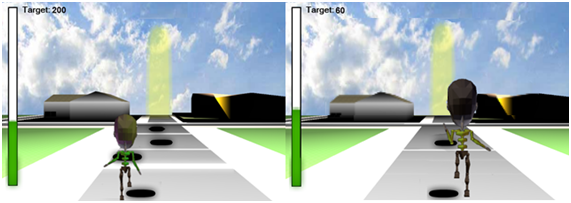
\includegraphics{ch1elderlypeople}
	\caption{Screenshoty HTML5 hry. Vlevo hraje nadaný hráč, vpravo s menší dovedností. \cite{8} }
	\label{ch1elderlypeople}
\end{figure}

\subsubsection{Jogging na dálku}

Ne každého baví běhat po parku samostatně a zároveň může být těžké najít někoho, kdo by si s vámi zaběhal ve stejnou dobu. Řešením může být jogging na dálku (jogging over distance), kdy dva lidé běží ve stejnou dobu, ale každý běží jinde, třeba i v jiném státě. Oba cvičící se dorozumívají přes telefon se sluchátky na hlavě. Povídají si, navzájem se podporují.

Různí lidé mají různou fyzickou kondici a může být problém se navzájem přizpůsobit v běhu tak, aby oba dva jedinci byli přibližně stejně namáhání. Neměla by nastat situace, kdy jeden udýchaně nemůže skoro mluvit a druhému naopak cvičení nic nedává.

V článku Balancing Exertion Experiences \cite{7} popisují svůj přístup k dané problematice. Každý z joggujících partnerů má při sobě chytrý telefon a měřič srdeční frekvence. Na telefonu mají nastavenou svojí ideální, cílovou srdeční frekvenci každý dle své fyzické kondice, případně dle doporučení doktora. Jestliže oba partneři mají srdeční frekvenci relativně stejnou vůči své cílové, pak je vše v pořádku. Partneři mohou běžet několik minut s cílovou srdeční frekvencí, poté se vyhecují, že na chvíli zrychlí a běží např. na 120\% své cílové frekvence. Pokud nastane situace, kdy první partner běží na 80\%, druhý na 110\%, jak vhodně donutit prvního zrychlit a druhého zpomalit? 

Autoři článku přišli se zajímavým řešením. Pomocí sluchátek mohou simulovat vjem, kdy se partneři slyší vedle sebe, kdy jeden slyší druhého před sebou, případně za sebou. Ve výše uvedeném příkladu by partner běžící na 110\% slyšel spoluběžce za ním, což by ho donutilo zpomalit. Opačně partner běžící na 80\% by slyšel toho druhého před sebou a byl by donucen zrychlit, aby se ve výsledku slyšeli co nejlépe, vedle sebe.

\subsection{Zdravotnictví}

Aplikace s adaptivní obtížností mohou pomáhat i nemocným lidem. Lidé po vážných úrazech se mnohdy učí, jak se vrátit zpět do normálního života. Při rehabilitaci lze mnohdy využít i počítačových her, které více motivují ke cvičení. Jestliže je taková hra příliš obtížná, pacient o ní brzy ztratí zájem. To platí i v opačném případě, kdy hra nutí pacienta provádět věci, které již bez problémů zvládá. Z těchto důvodů je velice vhodné obtížnost adaptivně měnit vůči konkrétním pacientům. Příkladem této aplikace je následující podkapitola Rehabilitace po utrpění mozkové mrtvice.

Druhá podkapitola v této sekci popisuje program asistující lidem trpícím demencí při jednoduchých úkolech.

\subsubsection{Rehabilitace po utrpění mozkové mrtvice}

Po cévní mozkové příhodě může dojít k částečnému až k v úplnému ochrnutí některých končetin. Pomocí různých cvičení lze tento dopad zvrátit. Mimo jiné mohou dobře posloužit jednoduché počítačové hry ovládané haptickým zařízením s adaptivním odporem a senzory. Obtížnost hry spočívá především v odporu ovladače a vzdálenosti, kterou musí osoba překonat. Jestliže se obtížnost zvolí špatně, hráč se může brzy nudit, být frustrován. V tom případě hru vypne a může být odrazen od další rehabilitace. Úkolem dynamického vyvažování hry je opět přizpůsobit hru různým lidem s různou rychlostí rehabilitace. \cite{9Pomdp} 

\subsubsection{Pomoc lidem trpícím demencí}

Lidé trpící nemocemi jako je Alzheimerova choroba potřebují pomoci i při běžných úkolech jako je mytí rukou. Tento proces lze rozdělit do několika podúkolů. Puštění vody, namydlení rukou, opláchnutí rukou, vypnutí vody, usušení rukou ručníkem. Někteří pacienti některé z kroků zapomínají, a poté jim je musí aplikace slovně připomenout. Cílem bylo vytvořit aplikaci, která se bude přizpůsobovat dovednostem aktuálního uživatele. Aplikace by neměla připomínat kroky mytí rukou, které pacient zvládne bez nápovědy provést sám. Připomínání všech kroků při každém mytí rukou by mohlo vést k jeho frustraci. \cite{10Dementia} 

\subsection{Výukové programy}

Existuje velké množství vzdělávacích programů a her. Jak takovou hru udělat, aby efektivně vzdělávala úplného začátečníka, ale i již pokročilého uživatele? I zde je prostor pro adaptivní přizpůsobování se programu uživateli. Představme si simulátor výuky v autoškole, kde by se dle schopnostech začínajícího řidiče měnilo prostředí. Na začátku by žák projížděl vesnicemi s minimálním provozem. Jak by se žák zlepšoval, přibýval by provoz, dopravní značky, semafory, vjel by do města apod. Jestliže by jel příliš rychle, v dalším úseku by se objevil retardér atd.

Ve sci-fi seriálu Stargate:SG1 ukázali možnost využití DDA při vojenském výcviku. Čím lépe si hrdina vedl ve virtuální realitě, tím více překážek mu bylo kladeno do cesty. \cite{11Stargate} 

Dále přiblížím komerční hru pomáhající s výukou na elektrickou kytaru a diplomovou práci o rozšiřování slovní zásoby předškolních dětí zábavnou formou.

\subsubsection{Výuka hry na elektrickou kytaru}

Známé herní vydavatelství Ubisoft vydalo během loňského podzimu hru Rocksmith, která má zábavnou formou uživatele naučit hrát na elektronickou kytaru. Oproti Guitar Hero, Rock Band neovládáte hru speciálním plastovým ovladačem, naopak využíváte opravdovou elektrickou kytaru, kterou připojíte přes speciální kabel do USB. Lze využít kytaru zakoupenou se hrou, nebo jakoukoli jinou.

V této výukové hře máte za úkol zahrát na kytaru správné akordy ve správnou chvíli. „Vše začíná jednoduchým brnkáním na jednu notu a pokračuje přes slajdy a příklepy k akordům a dalším složitějším technikám.”\cite{12RocksmithRev} Tímto lze popsat statickou část obtížnosti, ale autoři se zaměřili i na dynamické vyvažování obtížnosti a sami to vyzdvihují ve svém propagačním videu.\cite{13RocksmithVid} Jestliže během hraní uděláte několik chyb po sobě, hra se zjednoduší. Např. místo každého tónu budete hrát pouze každý třetí.

\subsubsection{Rozšiřování slovní zásoby}

Peter Peerdeman se ve své diplomové práci Intelligent Tutoring in Educational Games\cite{14Haas} zabýval využitím DDA u výukových her. Vytvořil hru Mijn naam is Haas(holandsky Moje jméno je Zajíc), která je zaměřena na mladší hráče, jež si mají rozšířit svojí slovní zásobu. Hlavní postavou ve hře je zajíc, který se stává průvodcem po hře. Hráč ovládá hru kreslením různých objektů do světa zajíce a hra se mu přizpůsobuje a dle nakreslených objektů vybírá další úkoly. Např. nakreslí-li několik mraků, začne pršet a dalším úkolem je nakreslit deštník, který by ochránil zajíce Haase před zmoknutím.

Hra při zadávání úkolů vhodně vybírá slovíčka dle úrovně hráče. Využívá se databáze 6000 slov, kde každé slovo je ohodnoceno číslem mezi 0 – 100 určující jejich obtížnost. Ohodnocení slova vyjadřuje kolik procent učitelů si myslí, že toto slovo je důležité znát žáky druhých tříd(groep  2)  základních škol v Holandsku. \footnote{Groep 2 navštěvují pětileté děti. Navštěvování první třídy ve 4 letech je dobrovolné, druhou třídu musí děti navštěvovat povinně. Číst, psát a počítat se začnou učit až v groep 3, která věkem dětí odpovídá prvním třídám v ČR. \cite{27EdHolland}} Lze předpokládat, že slova s hodnotou 90-100 žáci již dobře znají a naopak slova ohodnocená 0 – 30 nejsou důležitá k naučení. Zbytek slov lze rozdělit do šesti úrovní obtížnosti. Obtížnost 1 obsahující slova s hodnotou 80 – 90 až po obtížnost 6 se slovy s hodnotou 30 – 40.

Zadání úkolu vždy obsahuje většinu slov dítěti dobře známých, zbylé tvoří prostor pro učení. Každý úkol má přiřazeno několik různě obtížných synonym a program vybírá nejvhodnější slovo dle úrovně hráče, které několikrát zopakuje v různých větách pro lepší pochopení jeho významu.

\section{Cíl diplomové práce}

\endinput
%%
%% End of file `ch01.tex'.

  \chapter{Obecné}


\section{Model architektury}

Ať už použijeme DDA s online nebo offline adaptivitou, implicitní nebo explicitní, je zde spousta společných rysů, a proto je na místě vytvořit obecný model architektury dynamického vyvažování obtížnosti. Ve všech případech se snažíme podchytit zjednodušený model hráče na základě jeho projevů ve hře, a poté tyto informace dodáme hře, která herní svět upraví k lepšímu zážitku hráče.

Jeden z možných modelů DDA znázorňuje obr. \ref{fig:ch2ddaarch}. V principu se zaznamenávají akce hráče a herní proměnné jako je např. počet životů hráče. Na základě těchto logů se vytváří model hráče, model jeho zkušeností, dovedností, preferencí a osobnosti. Model hráče v kombinaci s aktuálním stavem hry slouží k odhadu očekávaného zážitku hráče v dalším stavu hry. A nakonec model zážitku s model výkonu hráče slouží jako vstup adaptačnímu a generačnímu enginu, který posléze upraví herní komponenty jakými je např. umělá inteligence NPC.

\begin{figure}
  \centering
  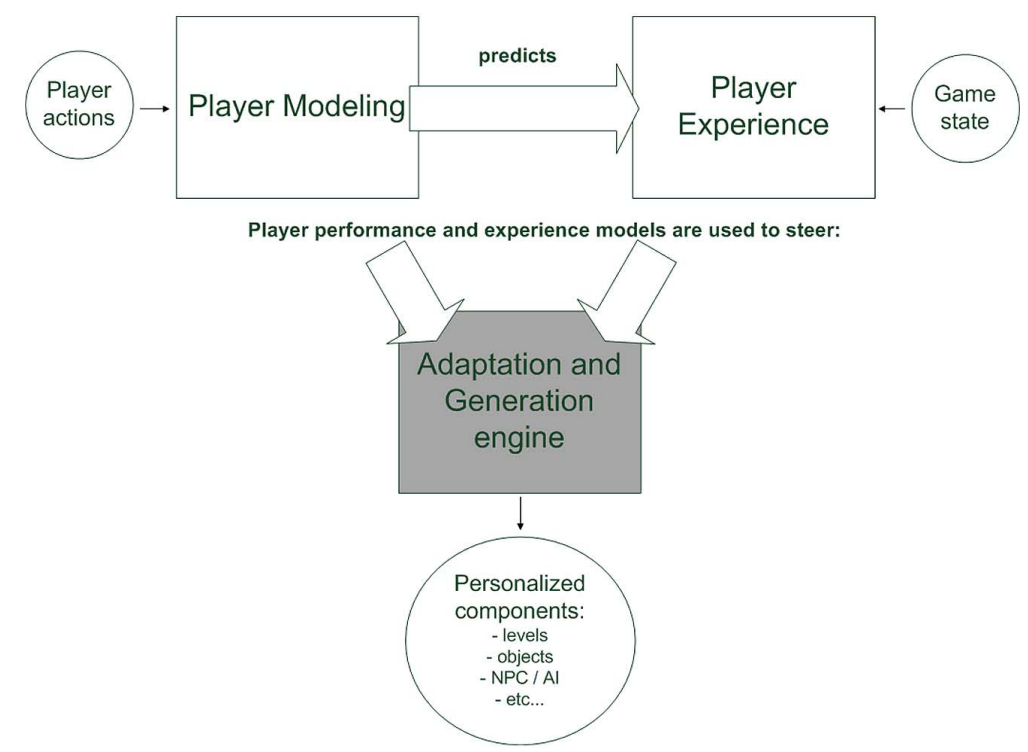
\includegraphics[width=0.75\textwidth]{ch2ddaarch}
	\caption{Přehled principů architektury adaptivních her. \cite{16Survey} }
	\label{fig:ch2ddaarch}
\end{figure}

V \cite{SwPatterns} se zabývali modelem DDA z pohledu návrhových vzorů objektového programování. Abstraktní model je znázorněn na obr. \ref{fig:ch2ddapatterns}. Senzory sbírají důležitá herní data, dle kterých se bude dále rozhodovat. Návrhový vzor Observer je připojen k Senzorům a v případě, že zaznamená zatelnou změnu v systému, vytvoří událost, trigger. Jednotlivé události jsou spojeny s akcemi a dohromady spolu tvoří pravidla uložená v databázi. V případě, že se spustí trigger spojený s akcí v některém z pravidel, rozhodne se v provedení této akce, což má na starost řadič, který má za úkol provést požadovanou změnu do stavu hry.

\begin{figure}
  \centering
  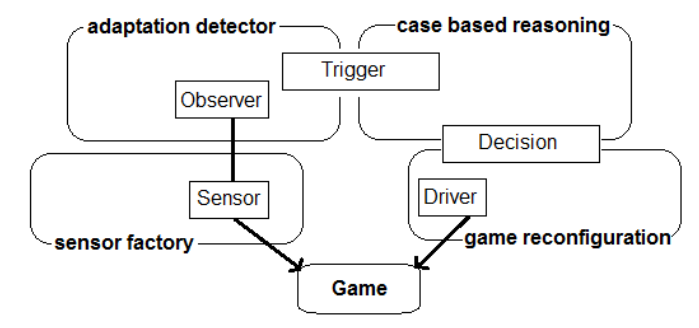
\includegraphics[width=0.75\textwidth]{ch2ddapatterns}
	\caption{Návrhové vzory DDA \cite{SwPatterns} }
	\label{fig:ch2ddapatterns}
\end{figure}

Dále se podíváme na jednotlivé návrhové vzory detailněji.

\subsection{Sensor factory}

Senzory jsou objekty, které pravidelně čtou herní data\footnote{Senzory nemusí zaznamenávat pouze herní data. Mohou zaznamenávat i prostředí uživatele např. pomocí Kinectu, nebo snímat aktuální tep hráče.} a upozorňují na změny zbytek DDA systému. Schéma návrhového vzoru znázorňuje obr. \ref{fig:ch2senzorfactory}. Senzor je abstraktní třídou, která zahrnuje periodické sbírání dat a upozorňující mechanismus. Konkrétní senzory z této třídy dědí a musí přepisovat abstraktní metodu refreshValue(), která zaznamenává konkrétní proměnnou systému. Třída SenzorFactory je zodpovědná za vytváření jednotlivých senzorů a je implementací návrhového vzoru factory. Továrna na senzory vyžaduje název senzoru a objekt, který má monitorovat. Vytvořené senzory si ukládá do registru. V případě, že uživatel zažádá o senzor, který už někdo vytvořil, dostane referenci na tento senzor. V opačném případě zkontroluje v ResourceManageru, jestli vytvořením nového senzoru se poruší některá z omezení zdrojů a pokud ne, senzor vytvoří.

\begin{figure}
  \centering
  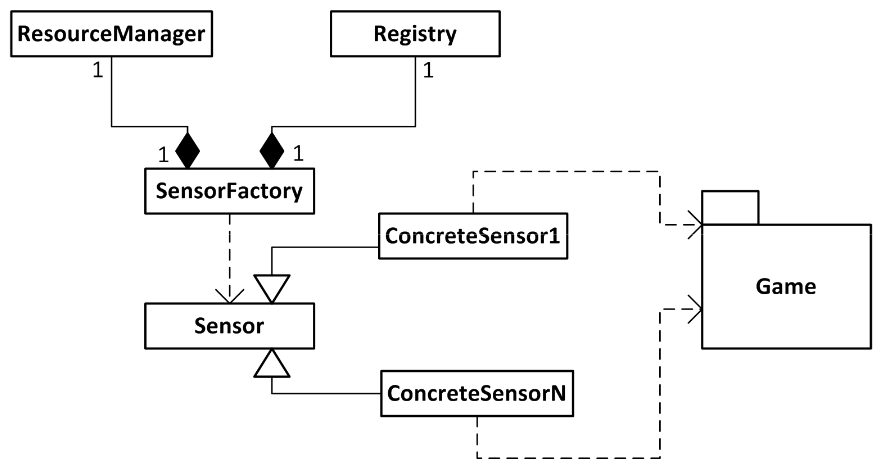
\includegraphics[width=0.5\textwidth]{ch2senzorfactory}
	\caption{Návrhový vzor sensor factory. \cite{SwPatterns} }
	\label{fig:ch2senzorfactory}
\end{figure}

\subsection{Adaptation detector}

Hrubá data získaná senzory se musí dále zpracovat. Tyto data získává AdaptationDetector pomocí observeru z návrhového vzoru senzor-observer. Na tomto místě se rozhoduje, jestli senzory již zaznamenaly dostatečnou změnu systému. Nedostatečnou změnou může být vystřelení jednoho náboje z plně nabitého revolveru. Naopak vystřílení půlky zásobníku může být významné. O významnost změny se stará TreshholdAnalyzer s Tresholdem. Treshold uchovává parametr hranice a její typ. (menší rovno, větší apod.) V případě dosažení prahu TresholdAnalyzer dá vědět AdaptationDetectoru, který vytvoří trigger, spouštěč. Trigger s sebou může nést další dodatečné informace jako je např. množství přeživších nepřátel. Viz obr. \ref{fig:ch2adaptationdesing}.

\begin{figure}
  \centering
  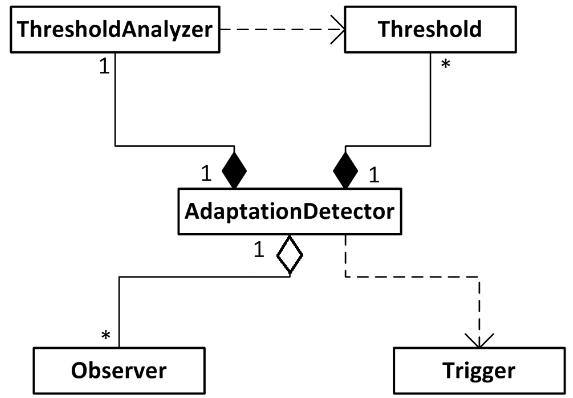
\includegraphics[width=0.5\textwidth]{ch2adaptationdesing}
	\caption{Návrhový vzor sensor factory. \cite{SwPatterns} }
	\label{fig:ch2adaptationdesing}
\end{figure}

\subsection{Case based reasoning}

Trigger spustí rozhodování na základě případů. Tento návrhový vzor(obr. \ref{fig:ch2casebase}) se použije, jestliže je možné vyvažování obtížnosti definovat konečným množstvím případů. InferenceEngine obsahuje dvě datové struktury: TriggerPool a FixedRules. Fixed rules obsahují pravidla, která jsou úzce spojená s konkrétní hrou. Pravidlo je kombinací triggeru a akce/rozhodnutí. TriggerPool funguje jako fronta událostí. Do fronty se řadí spuštěné triggery a jsou obsluhovány od nejstaršího. InferenceEngine vždy odebere jeden trigger z poolu, najde ho v databázi FixedRules pravidel a s ním nalezne vhodné rozhodnutí, které se má dále provést.

\begin{figure}
  \centering
  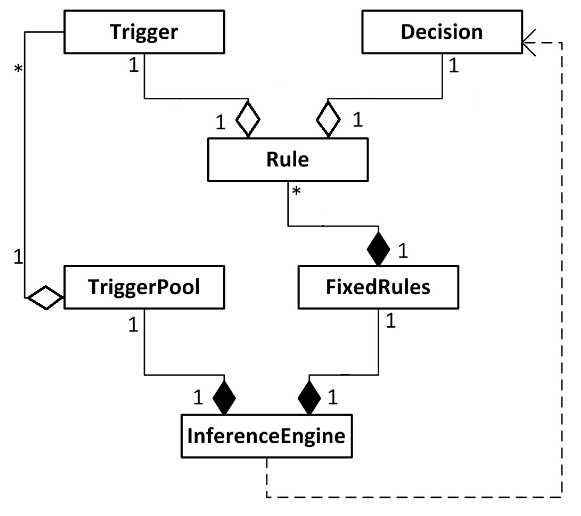
\includegraphics[width=0.5\textwidth]{ch2casebase}
	\caption{Návrhový vzor Case based reasoning. \cite{SwPatterns} }
	\label{fig:ch2casebase}
\end{figure}

\subsection{Game reconfiguration}

Posledním krokem je provedení požadované změny v herním světě. Návrhový vzor Game reconfiguration(obr. \ref{fig:ch2gamereco}) v sobě obsahuje jiný návrhový vzor, adapter. AdaptationDriver dostane ke zpracování rozhodnutí z InferenceEnginu. AdaptationDriver provede rozhodnutí za pomoci Driveru. Driver mění objekty, jež implementují rozhraní State, přes které zjišťuje aktuální stav objektu. S provedením jeho změny čeká dokud se nestane objekt neaktivním.

\begin{figure}
  \centering
  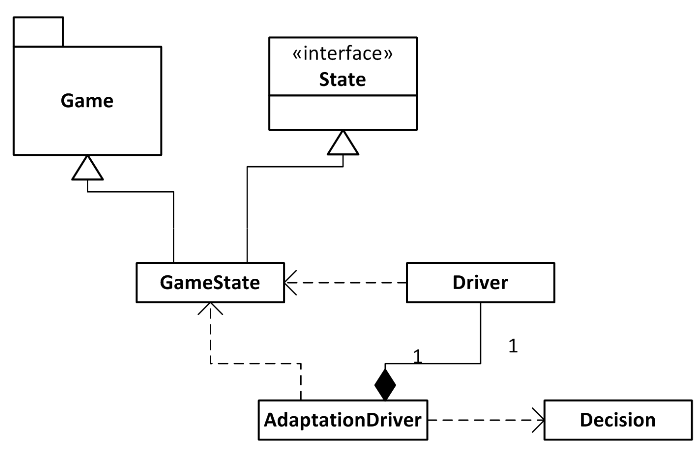
\includegraphics[width=0.5\textwidth]{ch2gamereco}
	\caption{Návrhový vzor Game reconfiguration. \cite{SwPatterns} }
	\label{fig:ch2gamereco}
\end{figure}

\section{Zábava}

Pojem zábava patří mezi velice subjektivní pojmy. Pro každého je zábavného něco jiného a svět her není výjimkou. Mezi hlavní zastupitele zkoumající tento pozitivní požitek patří Mihaly Csikszentmihalyi, který ideální stav maximální zábavy, maximálního ponoření do některé z činností nazval flow. Blíže tento stav bude popsán v následující podsekci.

Přestože se jedná o pojem subjektivní, pro použití DDA je nutné najít některé složky zábavy, které jsou změřitelné, kvantifikovatelné. Musíme být schopni zábavu měřit. Jestliže ji dokážeme změřit, můžeme to využít pro stavbu DDA algoritmů a i pro měření kvalit různých algoritmů mezi sebou. Možné metriky budou popsány dále.

\subsection{Flow}

Flow (tok) je stav mysli, kdy je osoba v průběhu provozování činnosti naprosto soustředěná, pociťuje nadšení, úspěch. „Flow je stav vědomí, kdy je člověk plně zaujatý svou činností. Nezabývá se jinými stimuly z okolí ani svými myšlenkami nebo pocity. Je naprosto soustředěný na prováděnou činnost. Dosahuje většinou, na své poměry, nadprůměrných výkonů, ale přitom mu to nepůsobí výraznou námahu. Je to harmonický zážitek, kdy tělo a mysl spolu bez námahy spolupracují. Tento stav je většinou spojen s pocity energie, radosti, harmonie a seberealizace.“ \cite{FlowCZ} S pojmem Flow prvně přišel zástupce pozitivní psychologie Mihaly Csikszentmihalyi ve své práci Flow: The psychology of optimal experience, česky vydané pod názvem O štěstí a smyslu života.

Požadovaný stav lze charakterizovat z pohledu dovedností člověka a náročnosti prováděné činnosti. Dosáhneme ho, jestliže provádíme úkol náročností odpovídající našim schopnostem. Viz obr. \ref{fig:ch2flow}. 

Jestliže se člověk seznamuje s novou činností, začíná v levém dolním rohu flow grafu. V tu chvíli nemá žádné dovednosti a pravděpodobně se začíná učit provádět činnost od jednoduchých částí po složitější. V knize \cite{OptimalFun} uvádí Csikszentmihalyi jako příklad takové činnosti hraní tenisu a vysvětluje to na obr. \ref{fig:ch2flow}. Alex začíná hrát tenis, a tedy se nachází ve fázi označené $A_1$. Alex v této chvíli neumí vůbec hrát tenis a začíná s tréninkem trefování se do míčku. Není to příliš obtížné, ale Alex si to užívá, protože náročnost tohoto úkolu přesně odpovídá jeho schopnostem.

\begin{figure}
  \centering
  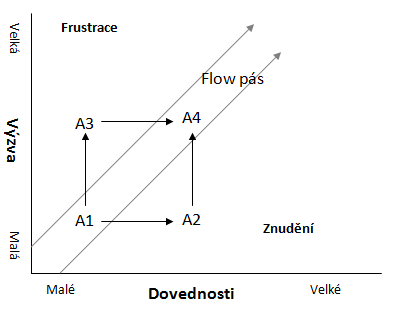
\includegraphics[width=0.5\textwidth]{ch2flow}
	\caption{Příklad pohybu jedince ve flow grafu. \cite{OptimalFun} }
	\label{fig:ch2flow}
\end{figure}

V této chvíli se Alex pohybuje v tzv flow pásu. Na stejném místě v diagramu nemůže zůstat Alex věčně. Jak danou činnost procvičuje, stává se v ní čím dál lepší, přestává ho to bavit, dostává se do nudy znázorněné v grafu $A_2$. V opačném případě se může stát, že potká zkušeného hráče. Hra proti němu je mnohem náročnějším úkolem a převyšuje Alexovy schopnosti. Alex se v takovém případě dostává do stavu úzkosti a stresu $A_3$.

V obou zmíněných příkladech se Alex nachází mimo flow pás a bude se snažit do něj opět dostat. V horším případě hru vzdá a další stav $A_4$ již v grafu nebude. V případě, že je ve stavu $A_2$, je dalším logickým krokem začít obtížnější úkol, vytyčit si nový cíl odpovídající jeho schopnostem. Ve stavu stresu $A_3$ má Alex jedinou možnost, zlepšit své dovednosti, aby se opět vrátil do flow pásu. Teoreticky může ubrat na výzvě, náročnosti úkolu, ale jak je jednou člověk vystaven takové výzvě, je pro něj těžké ji ignorovat a vzdát se jí. \cite{OptimalFun}

Dle Csikszentmihalyi se flow skládá z devíti elementů. \cite{FlowEng} Ne všechny jsou nutně potřebné k dosažení stavu flow.

\begin{enumerate}
	\item Jasné cíle
	\item Zpětná vazba
	\item Vyrovnanost náročnosti úkolů a schopností
	\item Splynutí činnosti a vědomí
	\item Koncentrace
	\item Žádné obavy z neúspěchu
	\item Pocit kontroly
	\item Změna vnímání času
	\item Vnitřní motivace
\end{enumerate}

Rozepisování jednotlivých bodů není záměrem této práce. Bližší informace lze nalézt např. na \cite{FlowEng}, \cite{FlowCZ}, nebo v originální knize \cite{OptimalFun}.

\subsubsection{Flow ve hrách}

Nás bude více zajímat napojení flow na vývoj počítačových her. Jenova Chen ve své diplomové práci Flow in Games\cite{thesisflow} vybral několik flow komponent, které označil za hlavní při návrhu hry. Dle Chena musí hra obsahovat následující tři elementy, aby hráč dosáhl stavu flow.

\begin{enumerate}
	\item Předpokladem je, že hra sama o sobě je pro hráče odměňující. Hráč sám o sobě chce hru hrát.
	\item Hra nabízí správnou náročnost úkolů vzhledem k hráčovým schopnostem, což mu umožňuje více se do hry ponořit.
	\item Hráč potřebuje cítit kontrolu nad prováděnou činností.
\end{enumerate}

Jsou-li splněny všechny tři body, hráč může ztratit pojem o čase a zcela se do hry ponořit.

Stavem flow ve hrách se dále zabýval Lennart Nacket, který ve svém článku\cite{FlowAll} shrnuje spojení flow s počítačovými hrami od různých autorů. Sweetserův a Wyethův herní flow osmi složkami vycházejícími z 9 složek flow od M. Csikszentmihalyi.

\begin{enumerate}
  \item Jasné cíle
	\item Zpětná vazba
	\item Výzva
	\item Hráčovi dovednosti
	\item Koncentrace
	\item Pocit kontroly
	\item Ponoření se do činnosti
	\item Sociální interakce
\end{enumerate}

\textbf{Jasné cíle} : 
Hráč by měl být vždy schopen kognitivně zpracovávat herní mise, úrovně, úkoly. Aktuální úkoly by měly být vždy jednoznačné a nematoucí. Hráč by měl být schopen vnímat svůj pokrok ve hře.

\textbf{Zpětná vazba} : 
Hra by měla vždy uživatele informovat o výsledku provedených akcí. Hráč by měl být seznámen, jak se blíží, či oddaluje od splnění cíle hry.

\textbf{Výzva} : 
U příliš jednoduchých her se nemohou uživatelé ponořit do hry. Hra musí být výzvou. Podstatné je rozlišovat náročnost ve formě špatně navrženého uživatelského rozhraní a ovládání a výzvu jako část herního designu. Špatné ovládání není nikdy žádoucí.

\textbf{Hráčovi dovednosti} : 
Hra by měla být navržena tak, aby hráči umožňovala efektivní získávání herních dovedností. Hra by měla brát v úvahu i možné dovednosti získané hráčem z jiných her.

\textbf{Koncentrace} : 
Hráč musí být do hry zcela ponořen, věnovat ji veškerou svojí pozornost.

\textbf{Pocit kontroly} : 
Hráč má mít pocit, že ovládá dění ve hře. Tento bod může být kritickým u návrhu DDA. Zjistí-li hráč, že jeho úspěch ve hře není zcela závislý na jeho výkonu, ztrácí pocit kontroly.

\textbf{Ponoření se do činnosti} : 
Podobné koncentraci. Hra má pohlcovat a udržovat hráče v maximální pozornosti, ale tak, aby mu to bylo stále příjemné.

\textbf{Sociální interakce} : 
Tento bod je přidán oproti prvotnímu flow. K dokonalému zážitku potřebuje člověk další lidské spoluhráče a protihráče.

\subsubsection{Zóna flow pro různé hráče}

Vraťme se znovu ke flow diagramu \ref{fig:ch2flow}. Dle příkladu s Alexem a jeho učením se tenisu by se mohlo zdát, že pro každého je ideální udržovat zcela vyrovnanou hodnotu schopností a náročnosti úkolů a udržovat uživatele v úzkém flow pásu, jak znázorňuje obr. \ref{fig:ch2flowzone1}.

\begin{figure}
  \centering
  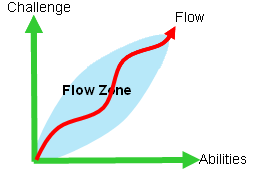
\includegraphics[width=0.5\textwidth]{ch2flowzone1}
	\caption{Obecně je vhodné hráče udržovat ve flow zóně. \cite{thesisflow} }
	\label{fig:ch2flowzone1}
\end{figure}	

Bohužel takový flow diagram nebere v úvahu individualitu hráče. Existují hráči, kteří mají rádi větší výzvy než jsou v tu chvíli schopni zvládnout, lze je nazvat hardcore hráči. Naopak existují příležitostní hráči, kteří netouží po velkých výzvách a nejraději se budou pohybovat lehce pod flow zónou. Těchto specifik si všímá např. práce \cite{RiskTakers}. Ideální průběh hry pro příležitostné/začínající hráče, běžné hráče a hardcore hráče znázorňuje graf na obr. \ref{fig:ch2flowzone2}. Mnohé práce tato specifika opomíjejí a často je jejich cílem upravit obtížnost hry, aby byl vyrovnaný počet hráčových výher a proher a už neberou v potaz, že někteří hráči přestanou hrát, když budou z poloviny pokusů prohrávat.

\begin{figure}
  \centering
  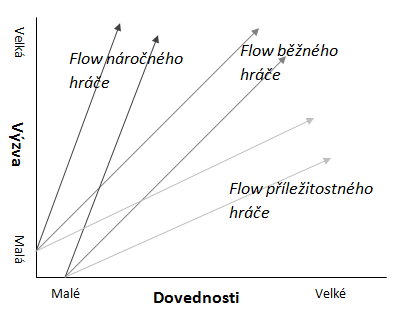
\includegraphics[width=0.5\textwidth]{ch2flowzone2}
	\caption{Flow zóna a specifika pro příležitostné a hardcore hráče. \cite{thesisflow} }
	\label{fig:ch2flowzone2}
\end{figure}	

\subsection{Metriky zábavnosti} \label{sec:defzab}

Hlavním cílem počítačových her je pobavení hráče. Může být tedy dobré umět zábavu přímo, či nepřímo změřit. Pro techniku DDA je existence takové metriky zcela zásadní. Bez ní by hra nevěděla, jakým způsobem se má přizpůsobovat hráči a neuměla by ohodnotit, jestli to dělá dobře. 

Metriky můžeme rozdělit do několika kategorií. Některé metriky jsou specifické pro konkrétní hru, jiné jsou obecně použitelné pro většinu existujících her. Dále jsou metriky, jež vycházejí pouze ze stavu hry, softwaru. Protikladem mohou být speciální metriky měřící hodnoty z vnějšího světa. Příkladem může sledování srdečního tepu \cite{7}. Dále lze využít webkameru, senzory na herních i neherních zařízení. Kromě tepu lze využívat např. pevnost stisku joysticku, měnící se odpor kůže, teplotu těla.\cite{16Survey} V této práci se pro naše účely zaměřím na metriky univerzálně použitelné a získané ze stavu hry.

Zábava ve hrách se často zjednodušuje do podoby náročnosti hry vzhledem k dovednostem hráče. Z tohoto důvodu velké množství přístupů pracuje s metrikami, které zábavu měří nepřímo, měří obtížnost hry. Často používanou metrikou je hodnota win-rate, poměr vítězstvích hráče ku jeho prohrám. Hodnota 0,5 značí polovinu výher a polovinu proher. Mnohé přístupy hodnotu 0,5 berou jako ideální. V tomto případě se hra snaží obtížnosti přiblížit co nejpřesněji dovednostem hráče. Jak bylo naznačeno v předchozí sekci, ne každý hráč ocení polovinu proher. Zde je prostor pro kombinaci statické a dynamické obtížnosti. Při statické obtížnosti si hráč vybere jednu z předem daných obtížností, např. začátečník, pokročilý, expert, kterým budou odpovídat hodnoty win-rate 25, 50, 75 %.

Další metriky využívají heuristiku, která numericky ohodnotí stav hry pro každého hráče a která nepřímo vyjadřuje pravděpodobnost výhry hráče. Samotná heuristika je herně specifická, ale prakticky u každé hry lze nějakou vymyslet, a proto jsou metriky, které ji využívají, obecně použitelné. 

V článku \cite{24DynLev} na základě zmíněné heuristiky přicházejí k třem metrikám. Počet změn ve vedení, napínavost během a konečný výsledek. Hráč, který dle heuristiky má největší pravděpodobnost na výhru je ve vedení. Jestliže se dostane do vedení jiný hráč, zaznamená se to. Metrika měří počet výměn hráčů během hry od začátku do konce. Je zde předpoklad, že hra je více zábavná, jestliže se hráči častěji ve vedení střídají, a tedy není pořadí hráčů stejné na začátku, během a na konci hry. Napínavost hry souvisí s rozptylem heuristiky pro jednotlivé hráče. Hra je napínavější, jestliže všichni hráči mají stejnou pravděpodobnost na výhru během celé hry. První z metrik počítá průměrnou napínavost během hry. Druhá udává o kolik vítěz vyhrál na ostatními hráči.

Všechny 4 zmíněné metriky (3 předchozí + win-rate) lze dobře využít v teorii her pro ohodnocení jednotlivých algoritmů a porovnání jich mezi sebou. Osobně mi počet změn hráčů na chvostu nepřijde jako dostatečný údaj. Mohlo by se stát, že každý z hráčů by byl během hry 2 krát ve vedení, ale jeden z nich by byl ve vedení 90\% času a zbylí hráči zbývajících 10\%. 5. metrika může znázorňovat dobu ve vedení pro každého hráče, nebo rozptyl těchto hodnot jako sjednocující údaj.

Jednou ze složek flow je kontrola. Hráč chce mít pocit vlády nad hrou. Jestliže budeme hru příliš často a hodně přizpůsobovat hráči, on/a si může všimnout, že nemá plnou kontrolu nad hrou, hra ho může přestat bavit. Proto by počet zásahů do hry měl být minimální. Spočítáme si pro každého hráče heuristiku pravděpodobnosti na vítězství vždy před adaptivním krokem $h_1$ a po něm $h_2$. Rozdíl $\Delta h = h_2 - h_1$ znázorňuje, jak moc jsme konkrétnímu hráči ublížili/pomohli k vítězství.  Můžeme vytvořit nové 2 metriky, kontrola a spravedlnost. Kontrola bude dána sumou absolutních hodnot $\Delta h$ během hry. Trochu paradoxně, čím menší hodnota kontroly, tím lépe. Tím méně bylo zasaženo do hry. Pro spravedlnost je důležité během hry pomáhat/ubližovat všem přibližně stejně. Čím vyrovnanější suma $\Delta h$ na konci hry mezi jednotlivými hráči, tím lépe.


	\chapter{Existující přístupy}

Dynamicky vyvažovaná obtížnost se zdá aktuálním tématem a možná v budoucnu zcela nahradí obtížnost statickou. Většina nalezených a citovaných článků byla napsána po roce 2000, velká část z nich vznikla až po roce 2010. Není tedy překvapením, že existující přístupy pro DDA pokrývají velkou část oblastí v AI obecně. Nalezneme zde částečně pozorovatelné markovské procesy, case-base reasoning, fuzzy logiku, evoluční algoritmy, neuronové sítě, mravenčí kolonie i příklady z teorie her.

Algoritmy můžeme zařadit do kategorií zmíněných v první kapitole. Klasifikaci jsem provedl na základě vědeckých článků, kde danou metodu použili. Ne ve všech případech bylo zařazení metod jednoznačné, a proto tabulka \ref{tab:klasifikacemetod} reflektuje i můj subjektivní názor. Tabulka může na první pohled vypadat podivně, stejný přístup je často označen za explicitní i implicitní nebo statický i dynamický. 

Explicitnost a implicitnost nevychází přímo z použité metody, ale záleží na designérovi, pro kterou z těchto kategorií se rozhodne. Z tohoto důvodu lze zařadit všechny zmíněné metody do implicitní i explicitní kategorie. Nikdy nemusí být hráč obeznámen s použitím DDA. Do explicitní kategorie jsem zařadil pouze evoluční algoritmus, POSM a dynamickou úroveň. Tyto přístupy pracují s hodnotou obtížnosti, která je snadno zobrazitelná uživateli s jejím jasným významem.

\begin{table*}[b]\footnotesize
\vspace*{0mm}
\caption{{\label{tab:klasifikacemetod}} Klasifikace metod do různých tříd. Mnohdy je zařazení nejasné, a proto je tabulka z části tvořena subjektivním pohledem.}
\vspace*{0mm}
\label{shadowtable}
\begin{center}
\begin{tabular}{| l || c | c || c | c || c | c | c |}
\hline
Metoda DDA & explicitní & implicitní & statická & dynamická & NPC & svět & úkoly \\
\hline
\hline
POMDP & & \checkmark & & \checkmark & & & \checkmark \\ \hline
Producent – konzument  & & \checkmark & \checkmark & \checkmark & \checkmark & \checkmark &  \\ \hline
Case-base reasoning  & & \checkmark &  & \checkmark & \checkmark & & \\ \hline
Fuzzy pravidla  & & \checkmark & & \checkmark & \checkmark & & \\ \hline
Evoluční algoritmus & \checkmark & \checkmark & \checkmark & & & \checkmark & \\ \hline
Mravenčí feromony  &  & \checkmark & & \checkmark & & & \checkmark \\ \hline
POSM & \checkmark & \checkmark & \checkmark & \checkmark & \checkmark & \checkmark & \checkmark \\ \hline
Dynamická úroveň  & \checkmark & \checkmark & & \checkmark & \checkmark & & \\ \hline
MCTS  & & \checkmark & & \checkmark & \checkmark & & \\ \hline
\end{tabular}
\end{center}
\end{table*}

Mimo evoluční algoritmus lze všechny metody zařadit mezi online algoritmy. Přístup producent-konzument je i offline algoritmem. Byl využit u střílečky z pohledu první osoby. Staticky je zde přizpůsobován svět, když do něho hráč vstoupí. Naopak dynamicky se upravuje přesnost a účinnost střelby nepřátel během boje. POSM patří k velice obecným přístupům. Vyžaduje na designérovi návrh konečného množství obtížností a algoritmus z nich posléze vybírá nejvhodnější obtížnost v danou dobu. Z tohoto důvodu je zcela na návrháři, jestli obtížnost bude měněna jen před začátkem hry na základě předchozích her, nebo bude měněna i v průběhu.

Poslední trojice kategorií představuje, čím je dána obtížnost hry. Ve většině případů upravovali umělou inteligenci protihráčů. Jak už bylo zmíněno, producent-konzument upravoval kromě NPC i svět, u POSM je volba obtížnosti na návrháři. Evoluční algoritmus byl využit pro generování úrovní do logické hry. POMDP spolu se simulací mravenců byly využity u vážných her. V obou případech se měnil druh úkolu dle jeho obtížnosti.

\section{Ne z teorie her}

\subsection{Částečně pozorovatelné markovské rozhodovací procesy} \label{sec:POMDP}

Částečně pozorovatelné markovské rozhodovací procesy (POMDP) byly úspěšně použity pro regeneraci rukou lidí po mrtvici \cite{9Pomdp} a u počítačového asistenta při mytí rukou člověkem trpícím demencí.

V obou případech byla osoba se systémem modelováno pomocí POMDP, které jsou schopné pracovat se sekvenčními dynamickými systémy, ve kterých jsou některé stavy preferované před jinými a ne vše související s procesem je plně pozorovatelné. V těchto případech nelze přímo pozorovat aktuální schopnosti uživatele.

V každém kroku je uložen belief state (pravděpodobnostní distribuce nad všemi stavy). Policy (politika) říká, kterou akci v daném kroku vybrat na základě aktuální belief state, které se na základě vybrané akce a nového pozorování aktualizuje.

\subsubsection{Influence diagramy}

Obecná POMDP mohou být řešena více exaktními způsoby, ale nejsou řešitelná s dostatečně krátkou odezvou pro naše využití. POMDP pro popsané úlohy může být redukováno na influence diagramy, které jsou snáze řešitelné.
 
Obecný influence diagram pro adaptivní systém si lze prohlédnout na Obr.~\ref{fig:ch3pomdp}. Apostrofované proměnné představují odpovídající neapostrofované proměnné v následujícím stavu. Např. hodnota napětí v následujícím stavu závisí pouze na hodnotách schopnosti a provedené akce z předchozího stavu.

\begin{figure}
  \centering
  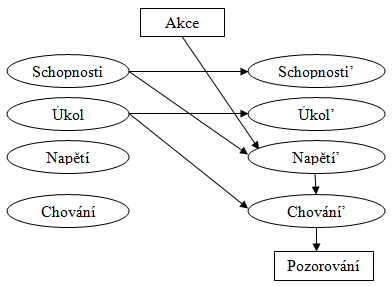
\includegraphics[width=0.5\textwidth]{ch3pomdp}
	\caption{Influence diagram pro adaptivní systémy}
	\label{fig:ch3pomdp}
\end{figure}

V každém kroku se provede právě jedna akce. Stav je popsán proměnnými 4 kategorií. Proměnná schopnosti(ability) je odhadem aktuálních schopností uživatele. Proměnná úkol(task) popisuje aktuálně prováděný úkol osobou. Proměnná napětí(stretch) znázorňuje náročnost aplikace vzhledem k aktuálnímu uživateli. Popisuje rozdíl úrovně obtížnosti zvolené akce a úrovně schopností jedince. Ideálně jsou úrovně shodné, napětí je nulové. Pokud je napětí vysoké, úkol je příliš obtížný. Jestliže je napětí záporné, úkol je příliš snadný. Proměnná chování(behavior) je přímo pozorovatelná. U pomocníka při mytí rukou je jím pozice rukou (ve vodě, na kohoutku atd.) a stav puštění vody.

\subsubsection{Příklad popisu stavu hry}

Pro lepší pochopení skupin proměnných a jejich významu uvedu příklady proměnných uvedených v článku \cite{9Pomdp}, rehabilitace po mozkové mrtvici.

Schopností je rychlost učení, jak rychle se každý uzdravuje. Úkol popisuje vektor n(r), kde pro jednotlivé hodnoty odporu ovladače je uložena maximální vzdálenost, kterou je osoba schopna dosáhnout. Napětí zde má zachován svůj význam z obecného popisu. Chování je zde nahrazeno celkovou únavou, která souvisí s následujícími pozorovanými veličinami. TTT, čas potřebný k dosáhnutí na cíl, CTRL, reprezentuje, jestli bylo cvičení vykonáno s pomocí kontroly, COMP, jestli si osoba snažila pomáhat vrchní polovinou těla místo využívání pouze její paže.

Konkrétní influence diagram můžeme vyřešit např. pomocí algoritmu PERSEUS, který najde v dostatečně krátkém čase přibližné řešení. Na základě pozorování a provedených akcí dokáže odhadnout schopnosti uživatele a vzhledem k tomu připravit odpovídající následující úlohu.

\subsection{Producent – konzument}

V mnohých hrách můžeme pozorovat vztah producent – konzument mezi světem a hráčem. Jestliže hráč získá ze světa moc prostředků, hra přestává být výzvou a naopak. Má-li hráč málo prostředku (např. munice, zdraví), může být frustrován kvůli vysoké obtížnosti.
Robin Hunicke popsala systém The Hamlet integrovaný do Half-Life SDK\cite{20Hun}, který vyvažuje obtížnost hry právě pomocí výměny zdrojů mezi světem a hráčem. Half-Life patří mezi klasické zástupce first-person shooter (FPS, „střílečky“).

\subsubsection{Použitá metrika}

Hunicke používá metriku pravděpodobnost smrti hráče. Ze série měření určí pravděpodobnostní distribuci poškození udělené hráči protivníkem během boje. Předpokládá Gaussovskou distribuci :

\begin{equation}
	   p(x)=\frac{1}{\sigma\sqrt{2\pi}}\mathrm{e}^{\frac{-(x-\mu)^2/2}{\sigma^2}}
\end{equation}

Pomocí určitého integrálu F(d) můžeme spočítat pravděpodobnost utrpění poškození menší, nebo rovnu d, kterou lze využít pro určení pravděpodobnosti přežití, jestliže má hráč aktuální zdraví rovné hodnotě d.

\begin{equation}
	   F(x) = \int_d^\infty p(x)\,\mathrm{d}x
\end{equation}

Dosazením za p(x) získáváme rovnici \ref{eq:integraldamage}.

\begin{equation} \label{eq:integraldamage}
	   F(x) = \frac{1}{\sigma\sqrt{2\pi}}\int_d^\infty \mathrm{e}^{\frac{-(x-\mu)^2/2}{\sigma^2}}\,\mathrm{d}x
\end{equation}

Tento integrál lze aproximovat funkcí erf z knihovny C++. V následujícím vzorci h odpovídá aktuálnímu zdraví hráče, $\mu, \sigma$ pro střední hodnotu a standardní odchylku poškození od aktuálního oponenta v nějakém čase t v budoucnu.

\begin{equation}
	   F(d_t) = 1-\frac{1}{2}(1+erf(\frac{h-\mu t}{\sigma\sqrt{2t}}))
\end{equation}

Během souboje se zaznamenává poškození d, které každý z protivníků udělí hráči. Na základě těchto hodnot a vzorců výše lze přibližně spočítat pravděpodobnost smrti hráče.

\subsubsection{Vyvažující strategie}

Systém Hamlet mění obtížnost na základě poptávky a nabídky. Na straně nabídky může systém zasáhnout umisťováním předmětů v herním prostředí (lékárničky, munice, zbraně). Dále může přizpůsobovat účinnost a přesnost hráčových zbraních, projev brnění apod.

Na straně poptávky manipulovat s nepřáteli (změnou jejich třídy, množství, počtu jejich životů, určením místa jejich objevení se na mapě). Stejně jako u hráče lze přizpůsobit sílu a přesnost jejich zbraní.

Autoři se snaží držet hráče v tzv. „komfortní zóně“, kdy se hráč cítí relativně v bezpečí. Jestliže se v průběhu boje zvedne pravděpodobnost úmrtí nad 40\%, Hamlet začne zasahovat do hry výše uvedenými způsoby.

Cílem této politiky je udržet zdraví hráče na střední hodnotě 60 se standardní odchylkou 15 bodů. Hamlet je navržen tak, aby pomáhal hráčům, kteří mají problémy, ale na druhou stranu, aby je neprotahoval za každou cenu skrz herní úrovně.

\subsection{Case-base reasoning} \label{sec:CBR}

Další možností pro implementaci DDA je Case-base reasoning. Rozhodování se v dané situaci dle úspěšné strategie použité v minulosti v situaci podobné.

Tento přístup využili Nizozemci u strategické hry Spring. \cite{21cbr} Proces celé adaptivní AI znázorňuje diagram Obr. \ref{fig:ch3cbrspring}.
Začne se sběrem dat (game observation). Proběhne simulace stovek her s různými hráči a vždy se v průběhu hry v určitých intervalech zaznamená zjednodušený popis stavu hry, použité strategie všech hráčů. 

Následuje offline zpracování (A. Offline processing), které může být časově náročné. Jednotlivé stavy se ohodnotí číslem (Game indexing). Dle předem známé heuristiky se určí, který z hráčů vede a „o kolik“. Kvůli velké paměťové náročnosti a posléze náročnosti vyhledávání v databázi se data komprimují pomocí shlukování (Clustering of observations). Situace hry navzájem si podobné se nahradí situací jednou.
 
\begin{figure}
  \centering
  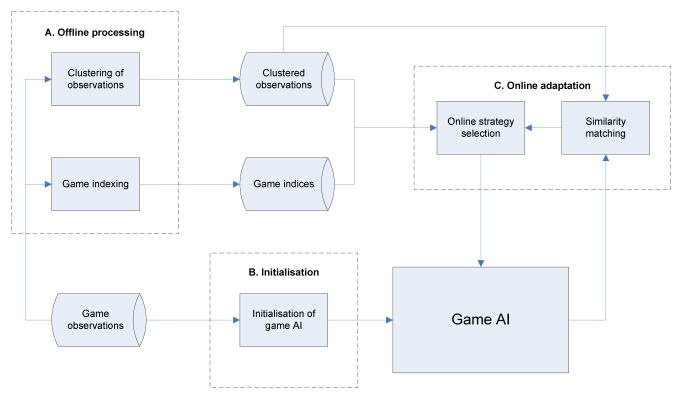
\includegraphics[width=0.5\textwidth]{ch3cbrspring}
	\caption{Proces adaptivní AI založené na CBR \cite{21cbr}}
	\label{fig:ch3cbrspring}
\end{figure}

Při inicializaci (B. Initialisation) se nastaví první strategie AI, která se ukázala nejlepší v daném scénáři. Poslední části schématu je online adaptace (C. Online adaptation), která nesmí být náročná na výpočetní výkon, jelikož se provádí v reálném čase. V určitých intervalech během hry se změní strategie hráče (Online strategy selection) na strategii, která se ukázala nejvhodnější v podobné situaci(Similarity matching).

\subsubsection{Sběr a úprava dat}

Při sběru dat pro adaptivní AI ve hře Spring získali 448 567 pozorování z celkem 975 her na třech různých herních mapách. Výsledná data zabírala 1192 MB nekomprimovaně. Spouštěli se vždy hry s dvěma protihráči. Pokaždé inicializováni různými strategiemi. V tomto kontextu se strategií míní vektor celkem 27 parametrů představující důraz na různé strategické chování na vysoké úrovni. Např. parametr aircraft\_rate ovlivňuje, jak moc často by měl hráč vytvářet vzdušné jednotky. Jakým způsobem se toho dosáhne už nesouvisí s těmito parametry. Dále je nutné popsat a uložit popis dané situace, jež se později použije pro vyhledávání podobných pozorování. Pozorování je popsáno 6 parametry. Fáze hry, síla materiálu, bezpečí velitele, ovládané území, ekonomická síla a počet vojenských jednotek.

\subsubsection{Ohodnocení her}

Každé z pozorováních se ohodnotí pomocí fitness funkce. Získané číslo určuje, kdo v dané chvíli vítězí. Fitness hodnota blížící se nule značí vyrovnané síly obou soupeřů. Vypočítá se např. z fáze hry, množství surovina a jednotek jednotlivých hráčů.

\subsubsection{Shlukování pozorování}

Shlukování je velice časově náročné, a proto se provádí offline. Cílem je nahradit více pozorováních jedním reprezentantem, který může být jedním pozorováním z původních dat, nebo pozorování vzniklé zprůměrováním podobných dat. Záleží na zvoleném algoritmu. Zde postačil dobře známý a jednoduchý algoritmus k-means.

\subsubsection{Inicializace hry}

V této fázi procesu se určí první strategie dynamické AI. Nejdříve se určí strategie, kterou využívá soupeř. Z ní se udělá abstrakce, jednotlivé hodnoty 27 proměnných se nahradí hodnotou z výčtu „málo“, „středně“, „hodně“.  Poté se naleznou v databázi pozorování s hráči podobnými soupeři a vybere se inicializační strategie, která si vedla nejlépe proti takovému hráči. Z tohoto důvodu nikdy není vybrána neefektivní strategie jako první.

\subsubsection{Online adaptace}

V průběhu hry se čas od času spustí adaptace herní strategie dle aktuálního stavu hry. Tato adaptace se skládá ze dvou částí, z porovnávání stavů a výběru strategie.

Podobnost dvou pozorování je rovna váženě sumě podobnosti šestice parametrů v jednotlivých pozorováních.

\begin{equation}
	   podobnost(poz1,poz2)=((1+f)*(0,5*u)) + mp + sc + cp + ep
\end{equation}

\begin{eqnarray*}
f &= &rozdilFazeHry(poz1,poz2) \\
u &= &rozdilPoctuJednotek(poz1,poz2) \\
mp &= &rozdilMaterialniSily(poz1,poz2) \\
sc &= &rozdilBezpecnostiVelitele(poz1,poz2) \\
cp &= &rozdilObsazenychPozic(poz1,poz2) \\
ep &= &rozdilEkonomickeSily(poz1,poz2)
\end{eqnarray*}

Samotná selekce nejvhodnější strategie se skládá ze tří kroků. Nejdříve se z databáze shluků vybere N nejbližších sousedů k aktuálnímu stavu hry dle výše uvedeného vzorce. Posléze se vybere menší podmnožina M stavů na základě herního indexu(fitness) dle zvoleného kritéria.

Zde se může projevit kombinace statické volby obtížnosti s dynamickou. Hráč si může před začátkem hry z volit jednu z pevně daných obtížností, např. lehká, normální, těžká. Vybere-li si běžnou obtížnost, bude algoritmus vybírat M stavů, jež mají fitness nejblíže k 0, která značí vyrovnané šance obou hráčů na výhru. Naopak hraje-li těžkou hru, algoritmus může vybírat pozorování s fitness odpovídající větší šance na výhru soupeřem.

Zbývá vybrat jedinou novou cílovou strategii. Z M stavů se vybere takový stav, kde strategie soupeře nejvíce odpovídá aktuální strategii soupeře v současné hře.

Na závěr nutno podotknout, že tento přístup nedává jistotu stejného chování a výsledku AI hráče jako ve vybrané hře z databáze. Při výběru se porovnávají pouze zjednodušené abstrakce stavu hry a navíc pouze s agregovanými shluky stavů. Výsledné chování hráče se může lišit od očekávaného.


\subsection{Fuzzy pravidla} \label{sec:fuzzy}

Máte-li umělou inteligenci ve své hře založenou na fuzzy pravidlech, může vás zajímat následující způsob tvorby adaptivní AI.

Základní myšlenka je jednoduchá. Mějme databázi fuzzy pravidel, kde každé z fuzzy pravidel může být aktivní, nebo vypnuté. Jestliže se hra jeví příliš těžká, vybere se některé z pravidel, a to se vypne. Naopak v případě, kdy se hra jeví příliš jednoduchá, jedno pravidlo se znovu aktivuje.

\subsubsection{Dead-end}

Autoři přístupu zvolili pro jeho testování hru jednoduchou hru Dead-end. Hráč je obklopen třemi stěnami a na čtvrté straně je východ. Jeho cílem uniknout tímto východem. Jeho snažení brání nepřátelské figury, které se naopak snaží hráče chytnout. Hráč má několik životů. Jestliže dojde ke kolizi hráče s nepřátelským duchem, jeden život ztratí. Ztratí-li všechny životy, hráč prohrává. Ve hře je navíc nastaven časový limit. Vyprší-li tento limit, hráč také prohrává. Naopak dostane-li se ven s alespoň jedním životem, vyhrává. Všechny postavičky se mohou pohybovat osmi směry.

Duchy lze rozdělit do dvou rolí. Duch nejníže vzhledem k souřadnici y tvoří předvoj a jistým způsobem ovládá ostatní duchy, obránce.

\begin{figure}
  \centering
  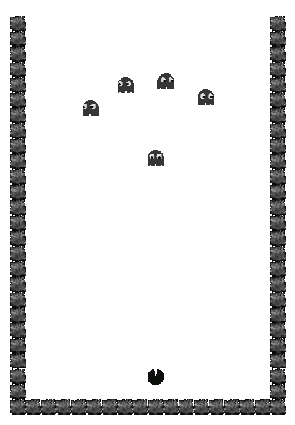
\includegraphics{ch3deadend}
	\caption{Screenshot ze hry Dead-End. \cite{25deadend} }
	\label{ch3deadend}
\end{figure}

\subsubsection{Fuzzy pravidla}

Duši se rozhodují na základě 5 vstupních fuzzy proměnných, jedné ostré proměnné a pěti výstupních proměnných.
Vstupními proměnnými pro pravidla předvoje jsou vzdálenost k hráči, vzdálenost k východu na ose y,  vzdálenost k hráči na ose x a binární proměnná, jestli duch už prošel kolem předvoje. Výstupními proměnnými jsou proměnné pro akce, které může duch provést – chytej hráče, nebo ustupuj od hráče.

Vstupní fuzzy proměnné pro obránce jsou vzdálenost k hráči, vzdálenost k předvoji, vzdálenost k nejbližšími jinému obránci na ose x a stejná binární proměnná značící, jestli byl už duch obejit.

Možné akce obránců jsou – chytej hráče, přibliž se k předvoji, oddal se od předvoje, oddal se od nejbližšího jiného obránce.
Příkladem fuzzy pravidla pro předvoj z kompletní tabulky 40 pravidel z \cite{25deadend} :
Pokud je hráč blízko předvoje a je blízko východu a hráč ještě neprošel kolem předvoje, pak chytej hráče velmi. Viz první pravidlo z následujícího obrázku Obr. \ref{fig-ch3fuzzytable}.

\begin{figure}
  \centering
  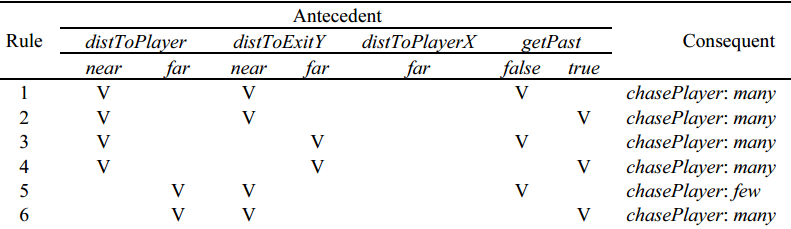
\includegraphics[width=0.75\textwidth]{ch3fuzzytable}
	\caption{Část fuzzy pravidel pro předvoj. \cite{25deadend} }
	\label{fig-ch3fuzzytable}
\end{figure}

Uvedené příklady fuzzy proměnných a pravidel by měli pro základní představu postačovat. Kompletní seznam fuzzy pravidel a detailnější popis jednotlivých proměnných včetně grafů funkce příslušnosti lze najít v již zmiňovaném zdroji \cite{25deadend}.

\subsubsection{Adaptivní změna počtu pravidel}

Jestliže se soupeř řídí všemi 40 pravidly, chová se velmi inteligentně. Hráč si na začátku hry může vybrat statickou část obtížnosti. Může ovlivnit požadovaný win-rate. Pokud tak neučiní, nastaví se win-rate na hodnotu 50\%. Každá hra trvá maximálně 20 vteřin. V případě, že hráč vyhraje a aktuální poměr vítězství/proher  je větší než cílená hodnota, hra se musí ztížit aktivováním momentálně vypnutého pravidla.

Naopak v případě, že hráč prohraje a aktuální hodnota win-rate je menší než cílená, hra je příliš těžká, zjednodušení proběhne deaktivací jednoho z pravidel.

Pokaždé, když se duch rozhodne dle jednoho z pravidel, zaznamená se to. Výsledný příspěvek se u pravidel obránců vydělí 4, jelikož jsou ve hře 4 obránci a jen jeden předvoj.

Pokud má dojít k deaktivaci pravidla, deaktivuje se pravidlo, které bylo využito nejméně krát, ale alespoň jednou. Kdyby se vyřadilo pravidlo, které se nevyužilo, hráč by nemusel vůbec změnu obtížnosti v příští hře poznat, jelikož by se mohli duchová chovat zcela stejně. Proč naopak nedeaktivovat pravidlo, které využíval soupeř nejvíce? V takovém případě by mohla být změna obtížnosti příliš drastická a mohlo by to vést k neočekávaným výsledkům.

Reaktivace pravidla je o něco složitější proces. Nejdříve se všechna pravidla rozdělí do skupin dle jejich konsekventů. Příspěvek celé skupiny pravidel je roven sumě příspěvků jednotlivých pravidel ve skupině. 

Poté se spočte suma vstupních příslušností hodnot pro každé z pravidel deaktivovaných dříve. Nakonec se zaktivuje pravidlo s největší sumou vstupních příslušností. Jestliže existují dvě pravidla se stejnou hodnotou sumy, zvolí se pravidlo jehož skupina má nejnižší příspěvek.

\subsubsection{Výsledky}

Na závěr připojuji jeden z grafů ukazující adaptivnost AI k třem různým hráčům s požadovanou hodnotou win-rate 75\% Obr. \ref{fig-ch3fuzzywinrate}. Ke srovnání na cílovou hodnotu došlo kolem 25. hry. 

\begin{figure}
  \centering
  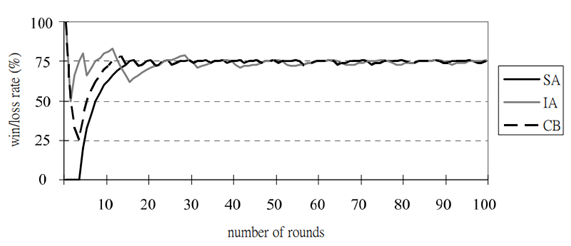
\includegraphics[width=0.75\textwidth]{ch3fuzzywinrate}
	\caption{Přibližování se k požadovanému win-rate 75\% během 100 kol proti třem různým hráčům. \cite{25deadend} }
	\label{fig-ch3fuzzywinrate}
\end{figure}

\subsection{Evoluční algoritmus} \label{sec:evol}

K zástupcům statické DDA lze bez váhání zařadit evoluční algoritmy (EA). Evoluční algoritmy zpravidla vyžadují velký výpočetní výkon, a proto nejsou vhodné pro realtime použití. Využitím EA pro DDA se zabývají např. články Automatic Generation of Game Elements via Evolution\cite{17Evol} a Making Racing Fun Through Player Modeling
and Track Evolution\cite{EvolTrack}. V prvním ze zmíněných článků využili EA pro generování různě obtížných úrovní logických her, naopak v druhém generovali závodní trať složenou z různých úseků.

\subsubsection{Generování bludišť}

V \cite{17Evol} byly testovacími hrami dva typy bludišť. V obou hrách byl stejný cíl, nalézt cestu mezi dvěma body. Obě bludiště dále sdílely hrací plán složený ze čtverců a nepřímo znázorněné překážky. Obtížnost hry je dána minimálním počtem kroků nutných k průchodu bludištěm. Neplatí zde zcela přímá úměra, obecně neplatí, že čím větší minimální počet kroků k dosažení cíle, tím je hra těžší. V případě, že bychom minimální počet kroků zcela maximalizovali, získáme bludiště, kde na začátku každý z tahů vede blíže k výhře. Hráč nemá dostatek možných tahů na výběr, a tedy je bludiště jednodušší než kdyby minimální počet kroků byl menší, ale naopak počet možných tahů by se zvýšil a ne všechny tahy by vedly blíže k cíli. Tuto hypotézu podporují informace získané při automatickém průchodu bludišť nutného pro ohodnocení obtížnosti hry. Algoritmus řešící bludiště se střední hodnotou minimálního počtu kroků pro daný typ bludiště běžel kratší dobu než pro bludiště s hodnotami blízkými minimu a maximu minimálnímu počtu kroků.

V první hře hráč pohybuje šachovou figurkou dle jejích platných tahů. Dále se na hracím plánu vyskytují nepřátelské šachové figury, které se nepohybují. Tyto figury ohrožují některá hrací pole. Jestliže hráč vkročí svou figurou na ohrožené hrací pole, prohrává. Jeho úkolem je figurku navést z její počáteční pozice do cílové a přitom nevkročit na žádné z ohrožovaných polí. Hráč nemá přímo označena ohrožená pole, musí využít své představivosti. Před generováním bludišť byly vždy pevně nastaveny druhy figur na hrací ploše, figura hráče a jeho startovní a cílová pozice. Cílem genetického algoritmu bylo rozmístit nepřátelské figury. Příklad jednoho bludiště na obr. \ref{fig-ch3evolchess}.

\begin{figure}
  \centering
  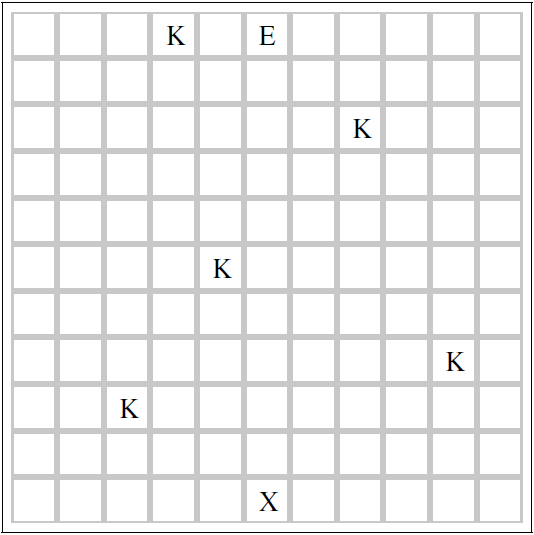
\includegraphics[width=0.3\textwidth]{ch3evolchess}
	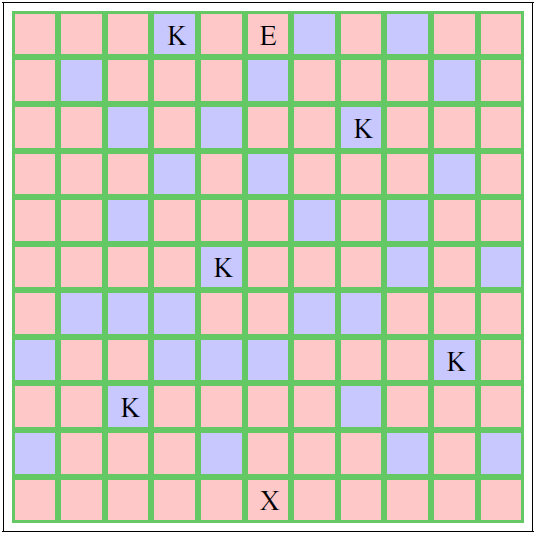
\includegraphics[width=0.3\textwidth]{ch3evolchess2}
	\caption{Příklad jednoho vygenerovaného bludiště se 6 jezdci a hráčem ovládajího věž. Vstup do bludiště je označen E, výstup X. Vlevo z pohledu hráče, vpravo znázorněné ohrožované pozice. \cite{17Evol} }
	\label{fig-ch3evolchess}
\end{figure}

Gen byl složen z pozic figur. Pro stejný druh figur nezáleželo na jejich pořadí. Bylo použito uniformní křížení. První ze dvou potomků má stejnou šanci pro získání pozice každé z figur jak od matky, tak i otce. Zbytek získá druhý potomek. Jestliže se po křížení nacházely u jednoho z potomků dvě figury na jedné pozici, potomci se zahodili, křížení se opakovalo. Při mutaci byla pozice jedné z figur náhodně přegenerována na ještě neobsazené pozice.

Druhou hrou bylo pestrobarevné bludiště. Každý čtverec bludiště má přidělenou jednu barvu z předem dané uspořádané množiny barev. Hráč se může mezi dvěma čtverci pohnout pouze v případě, kdy přechází mezi čtverci s barvami stejnými, nebo sousedními v rámci uspořádání. Opět při nepovoleném tahu hráč prohrává.

Gen je zde tvořen celým bludištěm uspořádaným po řádcích do jednoho řetězce o délce počtu čtverců bludiště. Bylo použito dvoubodové křížení a při mutaci se náhodně vybral jeden čtverec a vygenerovala se mu nová barva dle uniformního rozdělení pravděpodobnosti.

U obou her EA pracoval se stálou (steady-state) populací a selekce rodičů probíhala metodou turnaje. Vždy bylo vybráno náhodně 7 jedinců z celé populace, dva nejlepší z nich byli vybráni pro křížení a noví jedinci nahradili nejhorší dvojici vybranou pro turnaj.

Byly použity dvě fitness funkce. První maximalizovala minimální počet kroků k vyřešení bludiště. Druhá měla parametr - cílovou hodnotu minimálního počtu kroků - a tato fitness funkce minimalizovala rozdíl skutečného minimálního počtu kroků od požadovaného. Pro výpočet této hodnoty autoři článku využili metodu dynamického programování.

\subsubsection{Generování tratě}

Cílem práce \cite{EvolTrack} bylo procedurální generování co nejzábavnějších tratí pro závodní hry. Autoři článku za základě vlastních zkušeností a zkušeností dotazovaných hráčů definovali, jaká by měla být závodní hra, aby byla zábavná:


\begin{itemize}
	\item Hráči rádi jezdí co největší rychlostí. Trať by měla umožňovat dosažení maximální rychlosti aut.
	\item Naopak pouze jízda po dlouhých rovných úsecích není zábavná. Trať by měla být určitou výzvou pro hráče.
	\item Příliš časté nehody také nejsou ideální. Trať by měla být výzvou tak akorát.
	\item Lidé mají rádi různorodé výzvy. Jednotlivé tratě by měly poskytovat dostatečnou variabilitu výzev.
	\item Ježdění ve smyku a skoky autem se zdají být jednou ze základních složek zábavy závodních her.
\end{itemize}

Pro zjednodušení se generovaná trať skládala s předem daného počtu stejně dlouhých úseků.\footnote{Délka úseku dána délkou střední čáry.} Úsek mohl být rovný, nebo zatáčkou vlevo, či vpravo. Každá ze zatáček měla na výběr mezi 3 ostrostmi zatáčky. Dále gen obsahoval jednu ze tří šířek konce úseku. Začátek úseku vždy musel odpovídat šířkou konci úseku předchozího. Poslední variabilitou bylo umístění překážky na jeden z krajů úseku, nebo doprostřed. Dalším zjednodušením bylo vypuštění podmínky na kruhové trati. Trať byla pouze virtuálně kruhová - na jejím konci se hráč teleportoval na začátek se stejnou rychlostí a směrem jízdy. Křížení genů nebylo využito. Mutace změnila náhodně jeden z úseků na nový dle uniformní pravděpodobnosti.

\begin{figure}
  \centering
  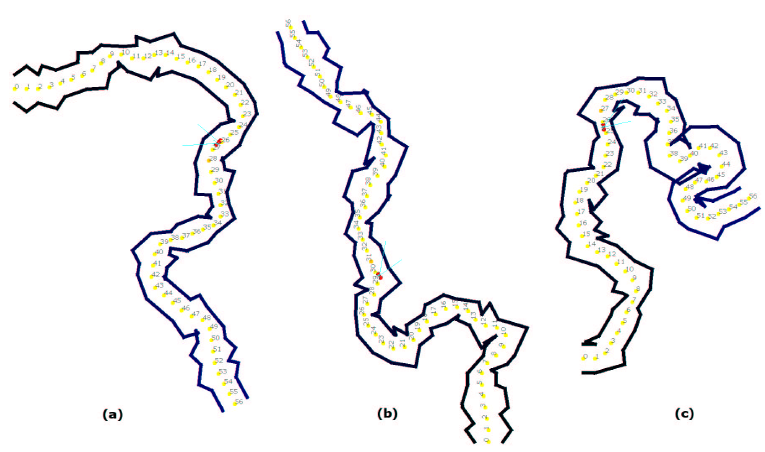
\includegraphics[width=0.75\textwidth]{ch3evoltrack}
	\caption{Příklad tří vygenerovaných tratí. První generována pro špatného hráče, druhá a třetí pro dobrého. Při generaci třetí tratě byla použita pouze jedna z fitness funkcí. \cite{EvolTrack} }
	\label{fig-ch3evoltrack}
\end{figure}

Metodou selekce byl kaskádový elitismus. Nejdříve se nagenerovalo 100 jedinců. Dle první fitness funkce se vybralo 50 nejlepších jedinců, kteří postoupili do druhého kola. V druhém kole se použila jiná, druhá fitness funkce, která vyřadila dalších 20 nejhorších jedinců. Ze zbylých 30 skončilo 15 nejlepších dle poslední třetí fitness funkce. První fitness funkci minimalizovala rozdíl cílené(předem dané parametrem) a skutečné hodnotě průměrné rychlosti na trati. Druhá fitness funkce maximalizovala maximální dosaženou rychlost na trati. Cílem bylo, aby trať obsahovala alespoň nějakou posloupnost rovných úseků. Poslední fitness funkce se zaměřila na měření množství výzev na trati. Vycházela z variance rychlosti na trati a počtu ujetých kol za danou dobu. 

Každá z vygenerovaných tratí byla vyzkoušena virtuálním hráčem nahrazující lidského hráče založeného na neuronových sítí. Vstupem do sítě byla aktuální rychlost, směr k dalšími checkpointu a 6 senzorů sledujících překážky.

\subsection{Mravenčí feromony} \label{sec:ants}

Optimalizace pomocí simulace umělých mravenčích kolonií patří mezi známé přístupy inspirované přírodou. Princip optimalizace mravenčími koloniemi je následující :


\begin{enumerate}
	\item Daný problém se vhodně modeluje jako graf skládající se z uzlů a hran mezi nimi
	\item Umělí mravenci se pohybují po hranách a zanechávají na nich feromon. Čím lépe si vedou, tím více feromonu zanechají.
	\item Mravenci se na každém uzlu rozhodují, kterou další hranou se vydají. S větší pravděpodobností zvolí hrany, na kterých je více zanechaného feromonu.
	\item Časem feromon vyprchává, je třeba obnovovat.
	\item Optimalizace končí, jestliže se ustálí cesty v grafu. 
\end{enumerate}

Tímto algoritmem se inspirovali vývojáři jedné ze serious games určené pro rehabilitaci částečně ochrnutých končetin lidí, jež utrpěli mozkovou mrtvici\cite{26poststroke}. Využití mravenčích feromonů je zde velice specifické a v tuto chvíli mě nenapadá jejich širší využití v jiné oblasti než rehabilitace částečně ochrnutých horních končetin, např. v zábavním průmyslu. Přesto je zde uvádím jako zajímavost, která stojí za zmínku.

Cílem práce bylo vytvořit hru, která budu procvičovat znovu ovládnutí pohybu ruky a zároveň bude svou obtížnost přizpůsobovat individuálním potřebám pacientů.

Výsledkem je jednoduchá hra odehrávající se na desce o rozměrech přibližně 1,5m na 1,5m rozdělená do buněk menší velikosti. Hra vždy označí některou z buněk za cílovou a pacient se jí má pokusit dosáhnout pomocí své ruky.

\subsubsection{Hráčův profil}

Schopnosti pacienta jsou zaznamenávány do tabulky Zóna schopnosti(ability zone). Zóna schopnosti je matice o velikosti m x n. Každá z buněk má přiřazeno reálné číslo reprezentující snadnost dosažení dané buňky. Cílem je vytvořit model obrazu schopností pacienta.
Tato definice pouze popisuje strukturu a zamýšlenou funkci zóny schopnosti, ale již nezmiňuje, jak takovou strukturu vytvořit. Existuje více různých cest.

Jednou z možností je uložit do každé buňky statistickou úspěšnost dosažení buňky pacientem, jestliže to dostal za úkol. Jinou možností jsou biologicky inspirovaní umělí mravenci.

Pacientova ruka představuje mravence, který se pohybuje po mřížce. Na místech, která navštíví, zanechá feromon. Feromon zanechá i na okolních buňkách, ale o něco méně. Čím více feromonu je na buňce zanecháno, tím je pro pacienta jednodušší této buňky dosáhnout, a proto je vhodnější cílit pacientovu ruku do buněk jiných.

\subsubsection{Zákon propagace}

Nově přidaná úroveň feromonu $level_s(c)$ na buňku $c$ mravencem s pozicí $s$ lze spočítat následovně.


\begin{equation}
	level_s(c)= \begin{cases}
											  A(1-\frac{dist(s, c)}{w}) & dist(s, c) \leq w \\
												0 & jinak
										 \end{cases}
\end{equation}

Ve vzorci konstanta $A$ značí nominální úroveň feromonu, jež se přidává na buňku s pozicí mravence, konstanta w značí dosah vlivu feromonu do okolních buněk. Funkce dist vrací vzdálenost mezi dvěma pozicemi předanými argumenty.

\subsubsection{Zákon vyprchávání}

Vyprchávání feromonů je též velice důležité. Zajistí zapomenutí oblastí, které hráč zasáhl pouze náhodou. Jelikož pacientovi pohyby nejsou plně kontrolovatelné, může se stát, že neúmyslně zasáhne některé buňky, které nechce.

Z tohoto důvodu chceme, aby vyprchávali více feromony, jež byly zasáhnuty náhodou. S vědomostí, které buňky zóny schopností pacient zasáhl pohybem po cestě p můžeme upravit množství feromonů na nich.

\begin{equation}
	F_{t+1} = F_t\frac{1}{vrcholyRychlosti(p)}
\end{equation}

Čím více vrcholů v grafu rychlosti na dané cestě, tím více byly pohyby trhané a tedy méně koordinované.

\subsubsection{Matice interakce}

Matice interakce je maticí m x n binárních hodnot. Jednička značí možnost vygenerovat cíl hry z odpovídající buňky, 0 naopak. V případě, že je náročnost hry odpovídající aktuálním schopnostem pacienta, matice interakce se nemění a generují se z ní nové cíle k dosažení rukou. Delší série výher značí, že hra je jednoduchá a hráč může být brzy z nuděn a nemotivován ke hře, k rehabilitaci a naopak delší série proher může způsobovat frustraci se stejným dopadem, koncem rehabilitace a možná i nechutí v ní v budoucnu pokračovat. V takovém případě se matice interakce musí přepočítat.

V obou případech se vypočítá pro každou z buněk jednoduchým vzorečkem gradient.

\begin{equation}
	grad(A_{i,j}) = \sum_{k \in \{i-1, i, i+1\}} \sum_{l \in \{j-1, j, j+1\}} A_{i, j} - A_{k, l}
\end{equation}

V případě příliš obtížné hry bude matice interakce obsahovat 1 na místech kladného gradientu, v opačném případě při příliš lehké hře bude obsahovat 1 v místech záporného gradientu. Příklad na Obr. \ref{fig-ch3feromons}.

\begin{figure}
  \centering
  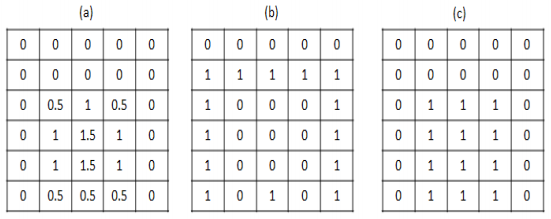
\includegraphics[width=0.75\textwidth]{ch3feromons}
	\caption{(a) Zóna schopností, (b) Interakční matice pro stížení hry, (c) Interakční matice pro zjednodušení hry \cite{26poststroke} }
	\label{fig-ch3feromons}
\end{figure}

První matice (a) obsahuje hodnoty zóny schopností po jednoduchém pohybu „zdola nahoru“ do buňky 3, 3. V matice (b) jsou jedničky na pozicích záporného gradientu dle výše uvedeného vzorce. V matici (c) jsou naopak jedničky na pozicích kladného gradientu. Z matic lze snadno vyčíst ztížení hry u matice (b) a zjednodušení u matice (c).

Jak jsem poukázal na začátku této kapitoly, jedná se spíše o zajímavost kvůli velmi specifickému užití metody mravenčích feromonů. Přesto je to inspirativní.


\section{Využitelné v teorii her}

\subsection{Částečně uspořádaná množina – Mistr}

Partially-Ordered-Set Master (POSM) \cite{22posm1} je obecně použitelným algoritmem pro dynamicky vyvažovanou obtížnost ve hrách. POSM lze využít kdykoli a v jakémkoli herním žánru. Jediným požadavkem na vývojáře je definovat konečné množství nastavení obtížnosti, pro které existuje relace „je těžší než“. Tento předpoklad není nerealistický. Většina her v současnosti obsahuje několik nastavení statické obtížnosti.

Oproti jiným přístupům DDA nevyžaduje modelaci chování hráčů. Nepředpokládá jiné znalosti o konkrétní hře. 
Základní princip algoritmu je jednoduchý. Mistr (program) inicializuje obtížnost na prostřední ze všech obtížností dle relace „je těžší než“ $\geq$. Odehraje se část hry. Posléze se určí, jestli mistr zvolil obtížnost správně dle schopností hráče, nebo jestli hra byla příliš těžká, nebo příliš jednoduchá. Na základě této informace upraví obtížnost hry správným směrem.

\subsubsection{Algoritmus POSM}

Vstupem algoritmu je částečně uspořádaná množina $(K,\geq)$ možných nastavení obtížnosti. Uspořádání je následující : $\forall i,j \in K$ píšeme $i>j$, pokud $i$ je více obtížné než $j$.
Po nastavení obtížnosti se odehraje kus hry a určí se hráčem pozorovaná obtížnost $o_t$.

\begin{itemize}
	\item $o_t=0$, jestliže obtížnost mistr zvolil správně a nemá se měnit
	\item $o_t=+1$, jestliže obtížnost byla příliš jednoduchá
	\item $o_t=-1$, jestliže obtížnost byla příliš těžká
\end{itemize}
	
Posledním vstupem algoritmu je učící konstanta $\beta\in(0,1)$. Čím blíže je konstanta hodnotě 1, tím je učení pomalejší, obtížnost je více statická.
Kroky algoritmu POSM:

\begin{algorithm}
\caption{Partially-Ordered-Set Master}
\label{posm}
\begin{algorithmic}[1]
\State $\forall k \in K : w_1(k) = 1$
\For{$i \gets 1, 2, \dots$}
	 \State $\forall k \in K : A_t(k) = \sum_{x \in K, x \geq k} w_t(x)$
	 \State $\forall k \in K : B_t(k) = \sum_{x \in K, x \leq k} w_t(x)$
	 \State $k_t = \operatorname{arg\,max}_{x \in K} \min({A_t(x), B_t(x))}$
	 \State Pozoruj reálnou obtížnost $o_t\in \{0,+1,-1\}$
	 \If{$o_t = 1$}
	   \State $\forall k \in K : w_{t+1}(k) = 
		                                        \begin{cases}
																						   \beta w_t(k) & k \leq k_t \\
																							 w_t(k) & jinak
																						\end{cases}
						 $
   \EndIf
	 \If{$o_t = -1$}
	   \State $\forall k \in K : w_{t+1}(k) = 
		                                        \begin{cases}
																						   \beta w_t(k) & k \geq k_t \\
																							 w_t(k) & jinak
																						\end{cases}
						 $
   \EndIf
\EndFor
\end{algorithmic}
\end{algorithm}

Na prvním řádku se inicializuje vektor w představující hodnoty „správnosti“ volby každé z obtížností. Na 3. řádku se uloží ke každé obtížnosti suma správnosti obtížností, které jsou těžší, nebo stejné než ona. Na 4. řádku se naopak uloží ke každé z obtížností suma správnosti obtížností, kterou jsou lehčí, nebo stejné než ona. Na pátém řádku se volí nová obtížnost dle uvedeného vzorce. Poté proběhne kus hry a algoritmus získá odpověď o reálné obtížnosti vzhledem k hráči. Na následujících řádcích se „správnosti“ jednotlivých obtížností vhodně upraví do další iterace hry.

\subsubsection{Příklad s balónky}

Algoritmus se lépe vysvětlí na příkladě.\cite{23posm2} Mějme jednoduchou hru sestřelování padajících balónků. Hráč je má sestřelit dříve než se dotknou země. Obtížností hry může být rychlost padání. Mějme předpřipraveno 10 různých rychlostí odpovídajících 10 nastavením obtížnosti.

Při inicializaci se vektor $w$ nastaví na 10 jedniček. Při prvním běhu bude vektor $A$ obsahovat $(10; 9; 8; 7; 6; 5; 4; 3; 2; 1)$ a vektor $B$ $(1; 2; 3; 4; 5; 6; 7; 8; 9; 10)$. Na 5. řádku se vybere náhodně 5. nebo 6. obtížnost, protože v obou případech :


	\[
	\max{\min{\{5, 6\}}} = \max{\min{\{6, 5\}}} = 5
\]

Po nastavení nové obtížnosti 5 může hráč hrát po předem stanovenou dobu, např. 15 vteřin. Na 6. Řádku se určí, jestli mistr dobře zvolil poslední obtížnost. V naší konkrétní hře, pokud hráč sestřelí všechny 95-100\% balónků, hra byla jednoduchá. Jestliže spadne na zem 5-15\% balónků, hra je vyvážená. Ve zbylých případech je hra příliš těžká.

V našem příkladu máme zkušeného hráče a při obtížnosti 5 sestřelil všechny balónky. Z toho vyplývá $o_t=+1$. Na řádcích 7 až 9 se provede úprava vektoru $w$. V tuto chvíli obtížnosti 1 až 5 nejsou vhodné, upraví se jejich správnost. Pro adaptivní konstantu $\beta=0,5$ bude vektor $w_2=(0,5;0,5;0,5;0,5;0,5;1,1;1;1;1)$.

Pokračujme druhou iterací. 

$A_2=(7.5;7,0;6,5;6,0;5,5;5,0;4,0;3,0;2,0;1,0)$, 

$B_2=(0,5;1,0;1,5;2,0;2,5;3,5;4,5;5,5;6,5;7,5)$

Pro přehlednost vektor minim z hodnot na odpovídajících si indexech.

$m=(0.5,1.0,1.5,2.0,2.5,3.5,4.0,3.0,2.0,1.0)$

Maximum z vektoru $m$ je hodnota 4.0, která je na 7. pozici. Hra se ztíží na 7. obtížnost.

Na uvedeném příkladě je vidět, že POSM je jednoduchým algoritmem s minimem předpokladů na znalosti konkrétní hry, a proto je použitelný pro velkou škálu užití. Vyzkoušen a testován byl např. na deskových hrách dáma a čínské šachy. \cite{23posm2}

\subsection{Dynamická úroveň}

Autoři tohoto přístupu se zaměřili na dynamické vyvažování obtížnosti v deskových hrách. \cite{24DynLev} Sami svůj algoritmus nijak nenazvali, tedy název této podkapitoly je mnou vymyšlen a google ho „nezná“. Alespoň ne ve spojitosti s tímto algoritmem.
Možnosti DDA v deskových hrách se od možností DDA v ostatních počítačových hrách výrazně liší. Ve střílečce, real-time strategii můžete obtížnost hry vyvažovat změnou pravidel hry aniž by si toho hráč všiml. Obtížnost může být dána přesností mušky botů ve hře, či množstvím zdrojů, s kterými soupeř pracuje ať už je během hry mohl, či nemohl získat.

Článek označuje jako jedinou možnost DDA v deskových hrách ovlivňovat AI soupeřů. Bohužel s tímto tvrzením nemohu souhlasit. I když se zaměříme pouze na deterministické deskové hry s úplnou informací, kterými jsou např. šachy, máme k dispozici online i offline dynamické vyvažování obtížnosti hry, které by jistě napadli většinu hráčů šachů, jelikož to již mnozí využili. Za offline DDA můžeme považovat odebrání některých herních figur před začátkem hry. K online vyvažování může patřit různé časové omezení na provedení tahu u jednotlivých hráčů. Vedoucí hráčů bude mít méně času na přemýšlení a tím se zvětší pravděpodobnost provedení chybného času a vystřídání hráčů ve vedení.

\subsubsection{Popis algoritmu}

Zpět k „dynamické úrovni“. Algoritmus má dva předpoklady k jeho využití. Vyžaduje funkci, jež umí ohodnotit všechny následující stavy ve hře. Hodnost vyjadřuje kvalitu dané situace z pohledu hráče, který je právě na tahu. Určuje šanci na výhru aktivního hráče.
Druhá funkce vrací status hry. Kdo vyhrává a jak moc. Kladné hodnoty statusu značí vedení, 0 remízu, záporné hodnoty prohrávání. Nejen znaménko statusu se bere v potaz, i hodnota je důležitá. Mělo by platit, že čím větší je hodnota statusu, tím větší šance na výhru daným hráčem.

Algoritmus je vytvořen pro dvouhráčové hry, kde jeden hráč má dynamickou úroveň. Při volbě nového tahu se řídí následujícími kroky:


\begin{enumerate}
	\item Uprav odhad soupeřovy úrovně na základě status funkce.
	\item Vygeneruj všechny možné následující stavy ze stavu aktuálního.
	\item Přiřaď hodnosti vygenerovaným stavům.
	\item Vyber následující tah jako nejvhodnější vzhledem k odhadované soupeřově úrovně.
\end{enumerate}

Pseudokód algoritmu by mohl vypadat následovně:

\begin{algorithm}
\caption{Dynamická úroveň}
\label{alg-dynlevel}
\begin{algorithmic}[1]
\State $level_1 \in \left\langle 0, 100 \right\rangle$
\For{$i \gets 1, 3, 5, \dots$}
	 \State $status_t = statusFnc(state_t)$
	 \State $level_t = \begin{cases}
											  0 & \text{pokud level} + \frac{status_t}{\alpha} < 0 \\
												100 & \text{pokud level} + \frac{status_t}{\alpha} > 100 \\
												level + \frac{status_t}{\alpha}  & \text{jinak}
										 \end{cases}
						 $
   \State $S_t = nextStates(state_t)$
	 \State $\forall s \in S_t : r_t(s) = rankFnc(s)$
	 \State $state_{t+1} = s, s \in S_t, \text{kde } r_t(s) \text{ je v } \frac{level_t}{100} \text{ pořadí seřazených s dle } r_t(s)$
	 \State $state_{t+2} = opponentTurn(state_{t+1})$
\EndFor
\end{algorithmic}
\end{algorithm}

Na prvním řádku se určí inicializační úroveň jako odhad úrovně soupeře. V článku[24] není přesně definováno, jak počáteční úroveň volit. Možností je náhodně generované číslo, případně statický výběr hráčem z několika předdefinovaných možností. Např. „lehká“ = 25, „střední“ = 50 atd.

Třetí a čtvrtý řádek slouží k novému odhadu úrovně oponenta. Figuruje zde konstanta $\alpha$, určující dynamičnost změny úrovně hráče. Konstanta je závislá na konkrétní hře. Může být volena experimentálně, nebo se může i v průběhu hry měnit např. pomocí algoritmu simulovaného žíhání.

Na řádcích 5 – 7 se vygenerují následující stavy a vybere se ten s nejvhodnější hodností dle úrovně soupeře. Příklad : existuje 20 možných tahů, které jsme ohodnotili a dle ohodnocení seřadili. Jestliže je úroveň rovna 75, zvolí se tah v $\frac{3}{4}$ seřazených tahů, tedy 5. Nejlepších tah. Po úroveň 50 se zvolí tah v polovině, tedy tah 10. ze seřazených tahů.
Na osmém řádku se počká na tah oponenta a celý cyklus se opakuje od začátku.

\subsubsection{Ohodnocovací a status funkce}

Jaký je rozdíl mezi rankFnc a statusFnc? Každá se využívá v jiné části algoritmu. Vnitřně mohou být stejné. Proč tedy autoři rozlišují funkce 2? V článku se k tomu obecně moc nevyjadřují, ale lze něco usoudit z jejich testovací hry Backgammon.
Ohodnocovací rank funkce je zde složitá a bere v úvahu mnoho parametrů popisujících stav hry. Parametry jsou např. počet kamenů již mimo hru, součet vzdáleností zbylých kamenů od konce, šance na zajetí svého kamenu soupeřem v příštím tahu, jsou-li všechny kameny alespoň ve 4. (posledním) kvadrantu hry apod.

Naopak status funkce popisuje stav hry méně složitě, více z lidského pohledu. Spočítá skóre každého hráče jako počet kamenů již mimo hru + suma vzdáleností zbylých kamenů od konce hry. Status je rozdílem těchto dvou hodnot.

\subsection{Monte-Carlo prohledávání stromu} 

Autoři z Pekingské univerzity vyzkoušeli spojení Monte-Carlo Tree Search(MCTS) algoritmu s dnes populárními neuronovými sítěmi. \cite{18Pac1}\cite{19Pac2}

V článcích upozorňují na nevýhodu tradičních metod DDA, kdy se obtížnost uměle mění např. přidáváním dalších a silnějších nepřátele, ale jejich inteligence zůstává stejná. Hráč se v takovém případě může cítit podveden. V Pekingu se vydali cestou dynamického vyvažování umělé inteligence a svůj přístup aplikovali na zjednodušené verzi známé hry Pac-Man.

\subsubsection{Pravidla hry Pac-Man}

Cílem hráče hrajícího za žlutou postavu Pac-Mana je sníst všechny kuličky v bludišti a zároveň se vyhýbat nepřátelům, duchům. Pac-Man zvítězí, jestliže sní všechny kuličky, duši zvítězí, jestliže chytnou Pac-Mana. Jestliže do 55 kroků žádná z těchto událostí nenastane, hra končí remízou. Oproti původnímu Pac-Manovi jsou ve hře další úpravy.


\begin{itemize}
	\item Bludiště je zmenšeno na velikost 16x16 a neobsahuje žádné Power upy.
	\item Ve hře jsou pouze dva duši místo původních 4 a mají stejnou rychlost jako Pac-Man. Z toho vyplývá, že jeden duch nikdy nemůže sám chytit Pac-Mana, duši musí spolupracovat.
	\item Pac-Man i duši se rozhodují pouze na křižovatkách. Jejich možné akce jsou jít vpravo/vlevo/nahoru/dolů, případně u křižovatek u kraje bludiště jejich podmnožina, procházení zdí je zakázáno.
\end{itemize}

\begin{figure}
  \centering
  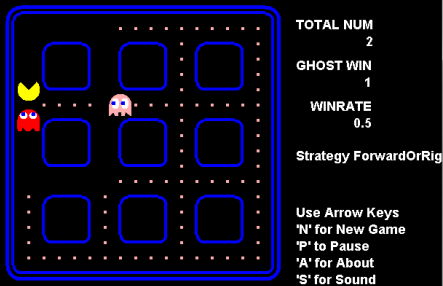
\includegraphics[width=0.5\textwidth]{ch3pacman}
	\caption{Zjednodušená verze Pac-Mana. Obrázek převzat z \cite{18Pac1}}
	\label{fig:ch3pacman}
\end{figure}

\subsubsection{Tvorba DDA pomocí MCTS}

Výkon umělé inteligence soupeřů založených na MCTS záleží na množství času, které MCTS poskytneme. Čím déle algoritmus běží, tím je pravděpodobnější inteligentnější chování duchů.

Pro účely simulace hráč Pac-Mana využíval ForwardOrRight strategii.
Pomocí opakovaných simulací s pevně daným simulačním časem získali závislost poměru vítězství (win-rate) na délce simulace. Několik získaných diskrétních hodnot proložili polynomem 4. stupně.

\begin{equation}
	y=-5,67*x^4+17,6*x^3-11,1*x^2-0,81*x+65,6
\end{equation}

V předchozí rovnici je x časem výpočtu MCTS v ms a y výsledné win-rate.
Běžný hráč chce vyhrávat přibližně v polovině případů. Vyřešením rovnice získáváme čas 105ms. Začínající hráč může upřednostnit častější vyhrávání, při win-rate 30\% (duchy) algoritmus potřebuje 28ms na výpočet.

\subsubsection{Využití neuronových sítí}
Další nevýhodou škálování AI pomocí změn simulačního času je horší využitelnost u real-time her, kde si nemůžeme dovolit věnovat stovky ms k výpočtu AI. Tento nedostatek lze odstranit využitím neuronové sítě místo MCTS.

Neuronovou síť se snažíme naučit chování odpovídající MCTS s daným simulačním časem. Při simulacích pomocí MCTS se při každém rozhodování duchů uložil stav hry, jako 23 proměnných a výsledné rozhodnutí o novém směru každého ducha.

Takto získaná data bylo použita pro učení neuronové sítě, která posléze nahradila původní algoritmus MCTS. Vstupními proměnnými byly např. pozice a směr hráče, pozice duchů a obsah sousedních dlaždic, vzdálenost mezi duchy a hráčem, čas simulace atd. Ve výstupní vrstvě bylo po 4 neuronech pro každého ducha, kde každý neuron představoval jeden zvolený směr.

Neuronové sítě odstranily časovou divergenci pro různé AI, ale naopak přinesly do systému jistou míru nepředvídatelnosti.

	\chapter{Vlastní přístup}

V této kapitole navrhnu vlastní inovativní přístup k dynamicky vyvažované obtížnosti. Mnou navržené algoritmy vychází z již existujících algoritmů teorie her a z tohoto důvodu se v první sekci této kapitoly věnuji základům z teorie her a popisu algoritmů, jež jsem převzal a upravil pro využití v DDA. V druhé sekci se již věnuji popisu vlastních algoritmů.

\section{Teorie her}

S teorií her se lze setkat především v ekonomické oblasti. Pro tuto sekci jsem vybral pouze témata z teorie her, jež budou využity. Nejdříve neformálně zadefinuji různé druhy her, hry v extenzivní formě a zero-sum hry. Následně nastíním algoritmy Minimax a Monte Carlo prohledávání stromu, které se používají pro hráče her v extenzivní formě.

\subsection{Základní definice}

\subsubsection{Dělení her}

Hry můžeme dělit dle obsahu nedeterminismu nebo dle úplnosti informace. U deterministických her je stav hry určen pouze rozhodnutím hráčů. Naopak u nedeterministických her je stav hry určen kombinací rozhodnutí hráče a projevu náhody. Mezi deterministické hry patří např. dáma a šachy. Naopak k nedeterministickým hrám se např. řadí hry využívající hrací kostku jako je Člověče, nezlob se.

Dle úplnosti informace dělíme hry na hry s úplnou a neúplnou informací. U her s úplnou informací všichni hráči znají kompletní stav hry a žádná informace jim není skryta. Naopak u her s neúplnou informací existuje část stavu neznámá všem hráčům. Mezi hry s neúplnou informací patří většina karetních her, kdy hráči neznají karty v soupeřově ruce.

\begin{table*}[b]\footnotesize
\vspace*{0mm}
\caption{{\label{tab:klasifikaceher}} Klasifikace her dle úplnosti informace a determinismu.}
\vspace*{0mm}
\label{shadowtable}
\begin{center}
\begin{tabular}{ l || l | l |}
 & S úplnou informací & S neúplnou informací \\
\hline
\hline
Deterministické & šachy, dáma & Hledač min \\ \hline
Nedeterministické  & Člověče, nezlob se & Prší \\ \hline
\end{tabular}
\end{center}
\end{table*}

\subsubsection{Extenzivní forma hry}

Hry v teorii her můžou být znázorněny ve dvou základních formách - normální a extenzivní forma. Hry v normální formě jsou používány pro hry, kde se hráči rozhodují současně. My budeme potřebovat formu vhodnou pro hry, kde se hráči ve svých rozhodnutích střídají a kde se rozhodují na základě dřívějších rozhodnutích. Průběh takové hry můžeme znázornit pomocí grafu. Tento graf se nazývá herním stromem. Graf je orientovaný s jedním kořenem a je bez cyklů. Uzly stromu představují možné stavy hry. Stav hry mimo jiné obsahuje informaci o hráči, který je na řadě. Hrany vedoucí z uzlu odpovídají všem možným tahům hráče, který je v daném stavu na řadě. Kořen představuje počáteční stav hry a listy stavy koncové. Všechny listy mají přiřazenou utilitu/zisk pro každého hráče. Jednoduchá utility funkce přiřadí hodnotu +1 výherci a -1 všem ostatním hráčům, v případě remízy přiřadí 0 všem hráčům.

Příklad herního stromu varianty piškvorek 3x3 Tic-Tac-Toe jen na Obr. \ref{fig-ttt-minimax}. V této hře se hráči pravidelně střídají, a proto uzly ve stejné hloubce odpovídají tahům stejného hráče. Aktuální hráč je v obrázku znázorněn vlevo. Ve spodní části jsou ukázány listy s utilitou pro hráče hrajícího křížky.

\begin{figure}
  \centering
  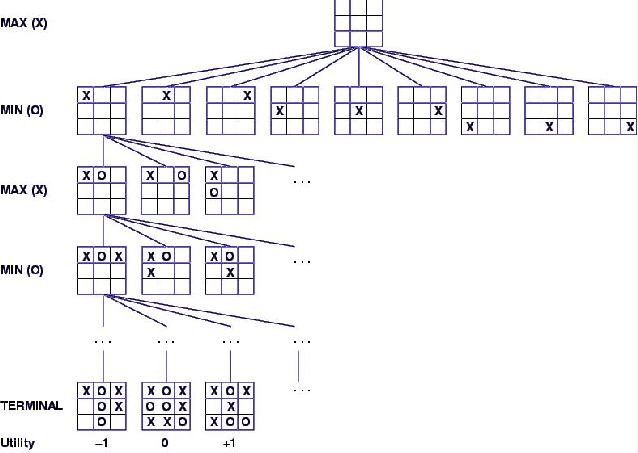
\includegraphics[width=0.75\textwidth]{ttt-minimax}
	\caption{ Výřez herního stromu hry Tic-Tac-Toe. }
	\label{fig-ttt-minimax}
\end{figure}

U nedeterministických her existují vnitřní uzly dvou typů. První odpovídá tahu aktuálního hráče stejně jako u her deterministických. Druhým typem je uzel náhody (chance node). Uzel náhody odpovídá stavu hry, kdy je na řadě náhodná událost - např. hod kostkou. Hrany z tohoto uzlu odpovídají náhodným jevům, možným stavům hry po náhodné události. Hrany jsou navíc ohodnocené číslem, které představuje pravděpodobnost jednotlivých náhodných jevů. V případě hodu kostkou budou všechny hrany ohodnoceny $\frac{1}{6}$.

U her s neúplnou informací hráči přesně nevědí, v jakém konkrétním uzlu herního stromu se nacházejí. Z jejich pohledu může být více uzlů představovat aktuální stav hry. Tato množina navzájem od sebe nerozlišitelných uzlů se nazývá informační množinou. Přestože hráč přesně neví, v kterém uzlu v rámci informačního stromu se nachází, může přiřazovat různé pravděpodobnosti jednotlivým stavům na základě předchozích tahů soupeřů.

Herní strom můžeme upravit pro hry s neúplnou informací. Uzel takového stromu nemusí představovat pouze jeden stav hry, ale celou množinu stavů, odpovídající informační množinu.

\subsubsection{Zero-sum hry}

Podkategorii her tvoří zero-sum hry. U těchto her platí, že součet utilit pro všechny hráče v každém listu se rovná 0. Tuto vlastnost využívají některé algoritmy, mezi které patří Minimax s alfa, beta prořezáváním.

U dvouhráčových zero-sum her můžeme pracovat pouze s utilitou pro jednoho hráče, utilita druhého hráče se snadno odvodí. Příkladem zero-sum hry je Tic-Tac-Toe. Z tohoto důvodu byla v herním stromu na Obr. \ref{fig-ttt-minimax} ukázána utilita pouze jednoho hráče.

\subsection{Algoritmy používané pro hry}

Existuje celá řada algoritmů umělé inteligence pro hry v extenzivní formě. V této podsekci popíši základní algoritmy Minimax s prořezáváním a Monte-Carlo prohledávání stromu, na jejichž základě navrhnu vlastní algoritmy pro DDA.

\subsubsection{Minimax}

V základní formě algoritmus Minimax pracuje pouze s dvouhráčovými zero-sum hrami. Každý z hráčů se snaží maximalizovat svojí utilitu a zároveň ví, že jeho soupeř se snaží jeho utilitu minimalizovat a tím maximalizovat utilitu svojí. 

Algoritmus prochází herní strom do hloubky až do listů. Ve chvíli, kdy získá vnitřní uzel utilitu ze všech potomků, vybere z utilit tu nejmenší/největší, kterou propaguje o patro výše. V soupeřově uzlu hráč vybírá minimum z potomků, ve svém uzlu vybírá maximum z potomků. Ve chvíli, kdy se dopropagují utility ze všech potomků ke kořeni, hráč vybere tah, který odpovídá uzlu s největší utilitou.

Ne vždy je možné procházet celý herní strom až do jeho listů. Často se omezuje maximální hloubka procházeného stromu. Jestliže algoritmus skončí v uzlu, který není listem, musí ohodnotit stav hry pomocí heuristické funkce a propagovat výše pouze odhadnutou utilitu. Heuristické funkce bývají herně specifické. Např. u hry dáma může být odhadnutá utilita rozdíl počtu zbývajících herních kamenů obou hráčů.

Rozšířenou variantou pro vícehráčové a ne nutně zero-sum hry je algoritmus MaxN. U těchto her se v listech stromu nenachází pouze jedna hodnota, ale každý hráč zde má svojí utilitu. Oproti základní verzi se zde propaguje výše celá skupina utilit. Každý hráč ve svém uzlu maximalizuje svojí utilitu.

\subsubsection{Alfa-beta prořezávání}

Alfa-beta prořezávání slouží k urychlení základního algoritmu Minimax aniž by to ovlivnilo jeho chování. Urychlení spočítá v prořezávání, neprocházení větví stromu, u kterých je již zřejmé, že nemohou obsahovat lepší tah pro aktuálního hráče v daném uzlu.

K ořezávání se používají proměnné alfa a beta. Alfa představuje maximální spodní hranici a beta naopak minimální horní hranici pro utilitu řešení v dané větvi herního stromu. V průběhu algoritmu se alfa může zvětšovat a beta naopak zmenšovat. Ve chvíli, kdy se překříží, si můžeme být jisti, že další expandování uzlu nepovede k řešení a další potomky neprocházíme.

Zrychlení algoritmu je silně závislé na pořadí procházení jednotlivých uzlů. Může výpočet až dvakrát zrychlit, ale může se stát, že se výpočet vůbec nezrychlí.

\subsubsection{Monte-Carlo prohledání stromu}

Jiným přístupem k vytvoření hráče je metoda Monte-Carlo prohledávání stromu. Oproti Minimaxu nepracuje s hotovým herním stromem. Herní strom si vytváří ve svém průběhu. Na začátku je herní strom tvořen pouze kořenem představující aktuální stav hry. Poté algoritmus v iteracích opakuje 4 kroky - selekce, expanze, simulace a zpětná propagace. 

Během \emph{selekce} se vybere list z částečně postaveného stromu. Při výběru se začne v kořeni a podle předem daného pravidla se volí potomci až se algoritmus dostane do listu. Vybraný list se \emph{expanduje}. Z listu se stane vnitřní uzel, přidají se mu potomci odpovídající možným tahům z daného stavu. Z každého přidaného uzlu se provede \emph{simulace} hry ideálně až do konce. Je nutné, aby simulace nebyla výpočetně náročná. Z tohoto důvodu se hráči volí tahy náhodně. Nakonec se výsledek hry \emph{propaguje} přes rodiče až do kořene.

\begin{figure}
  \centering
  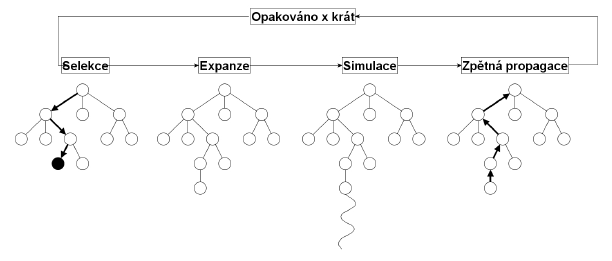
\includegraphics[width=0.75\textwidth]{ch4mcts}
	\caption{ Schéma jedné iterace MCTS. }
	\label{fig-ch4mcts}
\end{figure}

Každý uzel stromu obsahuje stav hry, aktuální aproximovanou hodnotu hry a počet navštívení uzlu během fáze selekce. 

Pravidlo pro selekci potomků není předem dáno. Jednou z často používaných metod selekce je UCT (Upper
Confidence bounds applied to Trees). Tato metoda se snaží vhodně vyvážit procházení slibných větví (s vysokou aktuální hodnotou) a procházení doposud málo navštívených uzlů. Každý z potomků je ohodnocen následujícím vzorcem:

	\[
	d_i = v_i + C * \sqrt{\frac{ln N}{n_i}}
\]

Poté se vybere uzel s největší hodnotou $d_i$ a proces se opakuje. Ve vzorci $v_i$ značí aktuální hodnotu i-tého potomka, $n_i$ počet navštívení potomka, $N$ počet navštívení rodiče. Pomocí konstanty $C$ se volí, jestli bude upřednostňováno procházení málo navštívených uzlů, nebo uzlů s vysokou hodnotou $v_i$. 

Volba počtu iterací je na programátorovi. Čím více iterací zvolí, tím lepšího chování dosáhne na úkor výpočetního času. Počet iterací nemusí být předem znám. Programátor se může rozhodnout pro ukončení algoritmu po určitém čase. Algoritmus má od konce první iterace vždy nějaké řešení, tah, který hráč má zvolit. Opakování iterací toto řešení zlepšuje.

\section{Algoritmy štěstí}



\subsection{E-HillClimber}

\subsection{Druhy}

\subsection{Treti}

\endinput
%%
%% End of file `ch01.tex'.

  \chapter{Testující prostředí}

Ahoj


\endinput
%%
%% End of file `ch01.tex'.

	\chapter{Provedené experimenty}

V této kapitole popíši provedené experimenty a ukáži naměřené výsledky, které následně zhodnotím.

Nejdříve budu hodnotit algoritmy zvlášť v rámci jednotlivých her. V poslední sekci kapitoly zhodnotím testované DDA algoritmy celkově.

Každý z experimentů obsahoval celkem 1000 iterací.

Jednotlivé metriky mají diametrálně odlišné rozsahy hodnot. Z tohoto důvodu v grafech zobrazuji místo konkrétních hodnot poměr k nejlepší hodnotě. Výběr nejlepší hodnoty závisí na druhu metriky. Změnu vedení a svobodu se snažíme maximalizovat, ostatní metriky minimalizujeme. Z tohoto důvodu u změny vedení a svobody zobrazuji poměr vůči maximu, u zbylých metrik je tomu naopak.

Pro jednodušší vizuální porovnávání algoritmů mezi sebou upravuji metriky, které se minimalizují. Pracuji s převrácenou hodnotou těchto metrik. Po této úpravě zobrazuji do grafů poměr k maximální převrácené hodnotě minimalizujících metrik. Z tohoto důvodu čím vyšší hodnoty pro každou z metrik, tím je algoritmus lepší.

\section{Bludiště}

Pro testování bludiště jsem nastavil jeho velikost na šířku a výšku 41 čtverců, maximální počet kroků 777. Koeficienty metrik byly nastaveny na 10 pro uvěřitelnost, 100 pro napětí, 500 pro náskok a 100 pro svobodu. Zbylé koeficienty byly nastaveny na 0. Výsledek si lze prohlédnout na následujícím grafu (\ref{fig-ch5mazehc}) a tabulce(\ref{tab-mazem}).

V grafu jsou použity zkratky pro použité algoritmy. E-HC představuje E-HillClimber, E-MM je pro E-MaxMax, E-MC pro E-MonteCarlo, POSM pro Částečně uspořádaná množina – Mistr a DL pro Dynamickou úroveň. U Bludiště nebyl použit E-MN pro E-Max$^n$. Algoritmus E-Max$^n$ má za úkol simulovat hráče. Hráč ve hře bludiště se rozhoduje pouze dle následujících stavů. Z tohoto důvodu zde je postačující Algoritmus E-MaxMax, který plní přesně stejnou funkci jako E-Max$^n$ u dalších her. Algoritmus Žádný představuje naměřené metriky z hry, kdy nebyl použit žádný DDA mechanismus. Slouží pro srovnání s DDA algoritmy.

\begin{figure}
  \centering
  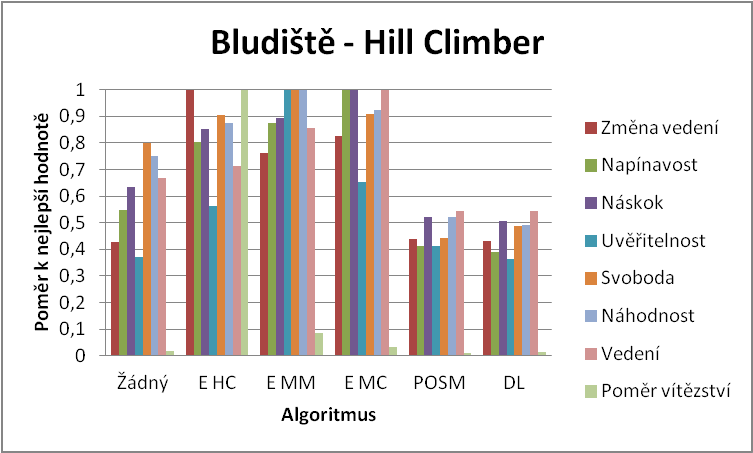
\includegraphics[width=0.75\textwidth]{ch5mazehc}
	\caption{Srovnání DDA alg. ve hře Bludiště s Hill Climber hráčem.}
	\label{fig-ch5mazehc}
\end{figure}

Z tabulky a především z grafu lze vyčíst, že algoritmy POSM a DL zaostávají nejen za ostatními DDA algoritmy, ale také za hrou, kde není použit žádný DDA mechanismus. Dopadají hůře i v metrikách napínavost a náskok, na kterých je testovali jejich autoři.

Při bližším zkoumání jsem zjistil, že důvodem pro špatné chování je absence přizpůsobování se metrice svoboda. Oba algoritmy příliš ořezávají možné tahy hráče na průměrných 7 tahů během hry. Bez použití DDA je průměrná hodnota svobody 12. Při nízké svobodě má hráč ve hře malé množství dveří, kterými by se vydal. Ve hře existuje málo větvení a naopak dlouhé chodby. Z tohoto důvodu se hráči rychle snižuje neprobádaný prostor - dlouhé chodby bez postranních dveří často odříznou část mapy od hráče. 

Oba algoritmy pracují pouze s hloubkou 1 a často se dostanou do situace, kdy už musí vytvořit chodbu k poslední bombě, přestože hráči zbývá ještě dostatek času. Případně nastane zcela opačná situace. Na mapě je více jak jedna bomba, tedy tyto algoritmy mohou bombu, ke které směřuje hráč, odříznout a udělat z ní falešnou, ale jelikož jsou ve hře především dlouhé nevětvené chodby, hráč se musí vrátit o velké množství kroků a vyprší mu čas.

\begin{table*}[b]\footnotesize
\vspace*{0mm}
\caption{{\label{tab-mazem}} Porovnání metrik zábavnosti u jednotlivých algoritmů ve hře Bludiště. Metriky změna vedení a svoboda se maximalizují, zbytek minimalizuje.}
\vspace*{0mm}
\label{shadowtable}
\begin{center}
\begin{tabular}{| l || r | r | r | r | r | r | r | r | r | r |}
\hline
Algoritmus & Počet kol	& Změna vedení & Napínavost & Náskok & Uvěřitelnost\\
\hline
\hline
Žádný & 93,127 & 8,217 & 343,6848421 & 239,851 & 81789,7937 \\ \hline  
E-HC & 114,905 & 19,176 & 233,9169735 & 177,951 & 53868,86 \\ \hline
E-MM & 113,32 & 14,64 & 214,5392914 & 169,935 & 30377,59274 \\ \hline
E-MC & 105,494 & 15,829 & 187,5847573 & 151,923 & 46656,61097 \\ \hline
POSM & 99,902 & 8,394 & 455,7661817 & 290,602 & 73884,68107 \\ \hline
DL & 95,431 & 8,29 & 483,7274291 & 300,486 & 83988,2358 \\ \hline
\end{tabular}
\end{center}
\begin{center}
\begin{tabular}{| l || r | r | r | r | r | r | r | r | r |}
\hline
Algoritmus & Svoboda & Náhodnost & Vedení &	Rozptyl Vítězů \\
\hline
\hline
Žádný & 12,19857537 & 15,05552294 & 33,04804979 & 0,121 \\ \hline  
E-HC & 13,79978394 & 12,92183276 & 31,00734155 & 0,002 \\ \hline
E-MM & 15,26174269 & 11,29628595 & 25,74151376 & 0,024 \\ \hline
E-MC & 13,84465841 & 12,22155687 & 22,05607333 & 0,065 \\ \hline
POSM & 6,76593984 & 21,72255666 & 40,54974306 & 0,176 \\ \hline
DL & 7,45030571 & 22,91638791 & 40,45994322 & 0,154 \\ \hline
\end{tabular}
\end{center}
\end{table*}

Algoritmy E-HC, E-MM a E-MC dopadly obdobně. Algoritmu E-HC se nejlépe dařilo v metrikách poměr vítězství a změna vedení, E-MM zvítězil v uvěřitelnosti, náhodnosti a svobodě, E-MC dopadl nejlépe v napínavosti, náskoku a ve vedení. Celkově nejlépe si vedl v této hře algoritmus E-MaxMax.

\subsection{Vzhled bludiště pro různé DDA algoritmy}

Druh použitého DDA algoritmu má velký vliv na výsledný vzhled bludiště. Typické zástupce vytvořených bludišť ukazuje obr. \ref{fig-mazes}. Pro bludiště vytvořené náhodně jsou typické zpočátku dlouhé chodby a posléze vyplňování chodbiček mezi dlouhými chodbami. Z vlastních algoritmů jsem vybral zástupce E-MaxMax, jehož bludiště působí nejpřirozeněji.

\begin{figure}
  \centering
  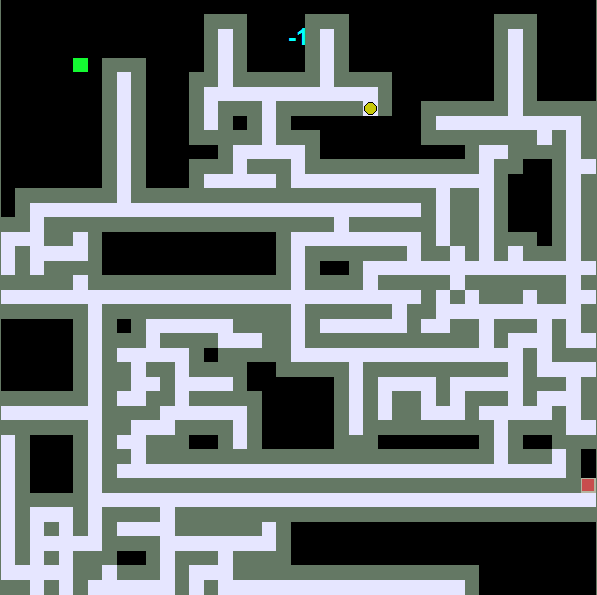
\includegraphics[width=0.35\textwidth]{mzadny}
	\hspace{3pt}
	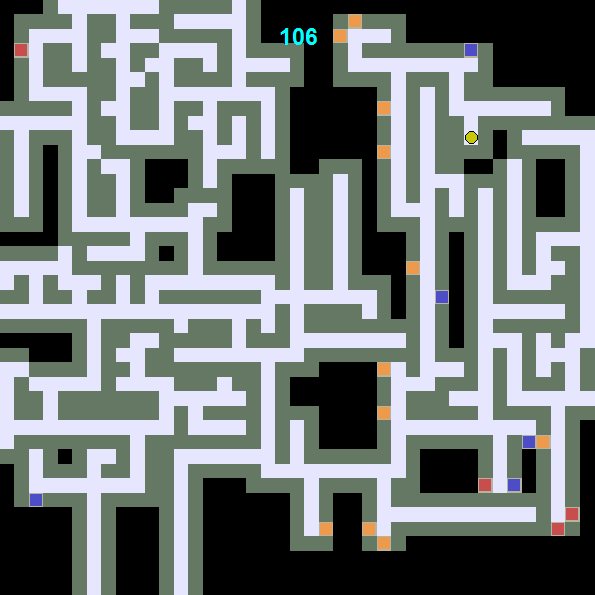
\includegraphics[width=0.35\textwidth]{mmaxmax} \\
	\vspace{6pt}
	\includegraphics[width=0.35\textwidth]{mposm}
	\hspace{3pt}
	\includegraphics[width=0.35\textwidth]{mdl}
	\caption{Srovnání bludišť vytvořených různými DDA algoritmy. Zleva-doprava, shora-dolů: žádný, E-MaxMax, POSM, DL}
	\label{fig-mazes}
\end{figure}

Bludiště vytvořená pomocí POSM a DL vypadají obdobně. Je pro ně typický výrazný počáteční kříž chodeb, kde algoritmy brzy uzavřou tři možné cesty a nechají mu jednu poslední.

\section{Ludo}

Oproti hře Bludiště je ve hře Ludo zásadní metrikou uvěřitelnost. V případě, že na tuto metriku nedáme důraz, HP nedovolí žádnému z hráčů hru vyhrát. Z jeho pohledu je ideální, když všichni hráči mají 3 figury v cíli a 4 těsně před cílem. Tato situace se mu zdá napínavá a ona by i ve skutečné hře byla, ale ne v případě použití falešné kostky. Z tohoto důvodu jsem nastavil koeficienty u uvěřitelnosti na 1000, spravedlnost, vedení, napětí na 10, náskok na 3 a svobodu na 1.

S tímto nastavením jsem provedl 3 experimenty. V prvních dvou hráli pouze dva hráči, jednou s algoritmem Hill Climber, podruhé s Max$^n$. Experiment s dvěma hráči jsem spouštěl, aby měly algoritmy Dynamický level a POSM prostředí, pro které byly navrhnuty - dvouhráčové hry. V třetí experimentu byly 4 hráči Max$^n$. První měl úroveň 50, další tři 100. Pro test DL a POSM jsem nahradil všechny 3 poslední hráče právě algoritmy DL, nebo POSM.

\begin{figure}
  \centering
  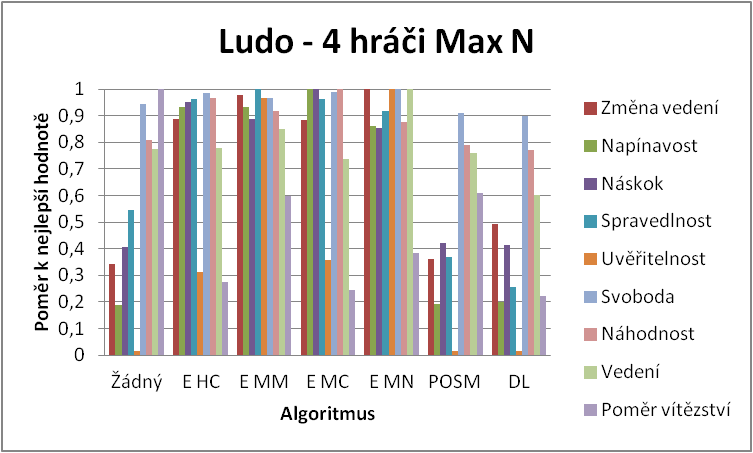
\includegraphics[width=0.75\textwidth]{ch5ludo4maxn}
	\caption{Srovnání DDA alg. ve hře Ludo se 4 Max$^n$ hráči. (úrovně 50, 100, 100, 100)}
	\label{fig-ch5ludo4maxn}
\end{figure}

Výsledky všech 3 experimentů byly obdobné. Zde uvedu pouze graf(\ref{fig-ch5ludo4maxn}) a tabulku(\ref{tab-ludom}) posledního experimentu. Grafy zbylých dvou experimentů lze nalézt v příloze.

\begin{table*}[b]\footnotesize
\vspace*{0mm}
\caption{{\label{tab-ludom}} Porovnání metrik zábavnosti u jednotlivých algoritmů ve hře Ludo. Metriky změna vedení a svoboda se maximalizují, zbytek minimalizuje.}
\vspace*{0mm}
\label{shadowtable}
\begin{center}
\begin{tabular}{| l || r | r | r | r | r | r | r | r | r | r |}
\hline
Algoritmus & Počet kol	& Změna vedení & Napínavost & Náskok & Spravedlnost\\
\hline
\hline
Žádný & 321,629 & 33,207 & 10,96064284 & 10,69 & 0,053439508 \\ \hline  
E-HC & 367,71 & 86,401 & 2,191965172 & 4,576 & 0,030182817 \\ \hline  
E-MM & 374,831 & 95,074 & 2,197616324 & 4,911 & 0,029112477 \\ \hline  
E-MC & 370,011 & 86,126 & 2,047674062 & 4,351 & 0,030268374 \\ \hline  
E-MN & 349,386 & 97,275 & 2,378575689 & 5,096 & 0,031668999 \\ \hline  
POSM & 329,262 & 35,024 & 10,57217622 & 10,292 & 0,079106286 \\ \hline  
DL & 342,281 & 47,836 & 10,26501397 & 10,484 & 0,113375705 \\ \hline  
\end{tabular}
\end{center}
\begin{center}
\begin{tabular}{| l || r | r | r | r | r | r | r | r | r |}
\hline
Algoritmus & Uvěřitelnost & Svoboda & Náhodnost & Vedení &	Poměr vítězství \\
\hline
\hline
Žádný & 24,57354378 & 1,86791164 & 1,189324764 & 67,3734372 & 0,021365861 \\ \hline  
E-HC & 1,226482879 & 1,95087896 & 0,996415593 & 67,020713 & 0,078176083 \\ \hline  
E-MM & 0,396586046 & 1,90887509 & 1,047952319 & 61,58128218 & 0,035686132 \\ \hline  
E-MC & 1,078624424 & 1,95431191 & 0,963174893 & 70,7910895 & 0,087272562 \\ \hline  
E-MN & 0,383798925 & 1,9757931 & 1,100121925 & 52,281059 & 0,055709066 \\ \hline  
POSM & 25,21722299 & 1,79829072 & 1,216838264 & 68,67222926 & 0,035035696 \\ \hline  
DL & 26,54645197 & 1,77747205 & 1,250394015 & 86,85364229 & 0,096187317 \\ \hline  
\end{tabular}
\end{center}
\end{table*}

Algoritmy POSM a DL měly zde již svou tradiční úlohu - ovládaly běžné hráče. Z tohoto důvodu neovlivňovaly metriky uvěřitelnost, svoboda, náhodnost a spravedlnost, které musely dopadnout podobně jako při nepoužití žádného DDA algoritmu. Oba zlepšily metriku změny vedení, ale zhoršily poměr vítězství. Náskok i napínavost měly podobnou, jako by se žádné DDA nepoužilo. 

U této hry a ještě více u Ztracených měst se projevil zásadní problém těchto DDA mechanismů. Pokud hráči jimi ovládaní jsou ve vedení, zhoršují svoje chování. Zhoršují ho až do zcela iracionální podoby. U hry Ludo se iracionální chování projeví např. v situaci, kdy hráč má jednu figurku před cílem a na kostce padla správná hodnota, aby hráč mohl přesunout svou figurku do cíle. V případě, že je hráč již dlouho ve vedení, tak raději nechá v figurku v potencionálně nebezpečné pozici a pohne figurkou jinou. 

Algoritmy E-HC, E-MM, E-MC a E-MN velmi předčily zbytek algoritmů i v metrice uvěřitelnost. V případě náhodného chování kostky se může s malou pravděpodobností stát, že padne jednomu hráči 6 třikrát po sobě. Je to relativně málo pravděpodobné, ale stát se to může. Algoritmy HP se snaží tyto málo pravděpodobné jevy eliminovat, a proto si dle metriky uvěřitelnost vedly lépe.

Celkově si nejlépe vedly E-MM a E-MN, které dokáží celkem věrně simulovat chování hráčů a následně se rozhodovat dle stavů hry dále v budoucnu. Mohou lépe naplánovat chování kostky z hlediska uvěřitelnosti a díky tomu se zaměřit více na ostatní metriky.

\section{Ztracená města}

I u Ztracených měst byla nejdůležitější metrikou uvěřitelnost. Bez ní prohrávající hráč získával postupně karty hodnot 10, 9, 8 atd. barev již vyložených expedic, dokud se nedostal do vedení. Nastavení koeficientů metrik jsem zvolil 1000 pro uvěřitelnost, 100 pro změnu vedení, spravedlnost, vedení a napětí, 10 pro svobodu a 0 pro náskok.

\begin{table*}[b]\footnotesize
\vspace*{0mm}
\caption{{\label{tab-lcm}} Porovnání metrik zábavnosti u jednotlivých algoritmů ve hře Ztracená města. Metriky změna vedení a svoboda se maximalizují, zbytek minimalizuje.}
\vspace*{0mm}
\label{shadowtable}
\begin{center}
\begin{tabular}{| l || r | r | r | r | r | r | r | r | r | r |}
\hline
Algoritmus & Počet kol	& Změna vedení & Napínavost & Náskok & Spravedlnost\\
\hline
\hline
Žádný & 51,21 & 5,17 & 169,3785106 & 159,11 & 2,97949985 \\ \hline  
E-HC & 51,652 & 6,219 & 90,11489792 & 109,66 & 2,083795471 \\ \hline  
E-MM & 51,058 & 15,105 & 35,89171719 & 92,52 & 2,51490921 \\ \hline  
E-MC & 51,076 & 6,763 & 84,52874032 & 106,63 & 2,407272356 \\ \hline  
E-MN & 51,284 & 16,647 & 34,66283799 & 78,3 & 1,853999951 \\ \hline  
POSM & 53,785 & 5,038 & 204,2092341 & 217,97 & 3,458477317 \\ \hline  
DL & 49,957 & 4,838 & 283,7280003 & 228,54 & 3,401727139 \\ \hline  
\end{tabular}
\end{center}
\begin{center}
\begin{tabular}{| l || r | r | r | r | r | r | r | r | r |}
\hline
Algoritmus & Uvěřitelnost & Svoboda & Náhodnost & Vedení &	Poměr vítězství \\
\hline
\hline
Žádný & 4,930532754 & 30,0635238 & 12,59686374 & 15,751 & 0,016 \\ \hline  
E-HC & 0,612039822 & 31,8330098 & 10,61479482 & 15,426 & 0,055 \\ \hline  
E-MM & 0,467313632 & 29,8150478 & 11,6301367 & 6,802 & 0,093 \\ \hline  
E-MC & 0,78408408 & 31,6226395 & 11,05890933 & 14,119 & 0,089 \\ \hline  
E-MN & 0,52395678 & 29,1162948 & 11,52272589 & 7,209 & 0,081 \\ \hline  
POSM & 4,956223714 & 27,4061938 & 12,97565858 & 16,7575 & 0,358 \\ \hline  
DL & 4,944157754 & 26,5193542 & 14,25249958 & 18,3885 & 0,408 \\ \hline  
\end{tabular}
\end{center}
\end{table*}

Opět byly spuštěny dva experimenty s různými v hráči. V jednom hráli proti sobě HillClimber IS s úrovněmi 50 a 100 a v druhém MiniMax IS se stejnými úrovněmi. Výsledky byly podobné, a proto se zaměřím na experiment se složitějšími hráči (graf \ref{fig-ch5lcmm}, tabulka \ref{tab-lcm}). Graf druhého experimentu lze nalézt v příloze.

DL a POSM opět ovládaly jednoho z hráčů, a tedy nemohly ovlivnit čtveřici metrik spravedlnost, uvěřitelnost, svoboda a náhodnost. Oba dva algoritmy dopadly špatně z důvodu nastíněného u hry Ludo. Ve Ztracených městech člověk dokáže snadno rozlišit zcela iracionální tahy od těch použitelných. DL a POSM ale mají tyto iracionální tahy k dispozici. Jestliže je hráč ovládaný DL nebo POSM ve vedení, nejrychleji srovná skóre vyložením nové expedice, za kterou má záporné body. Bohužel takový tah může být zásadní a i kdyby posléze hrál daný hráč dokonale, nemusí mu to stačit k opětovnému dostání se do vedení. Z tohoto důvodu je u Ztracených měst lepší nepoužít žádný algoritmus než POSM a DL v nezměněné podobě.

\begin{figure}
  \centering
  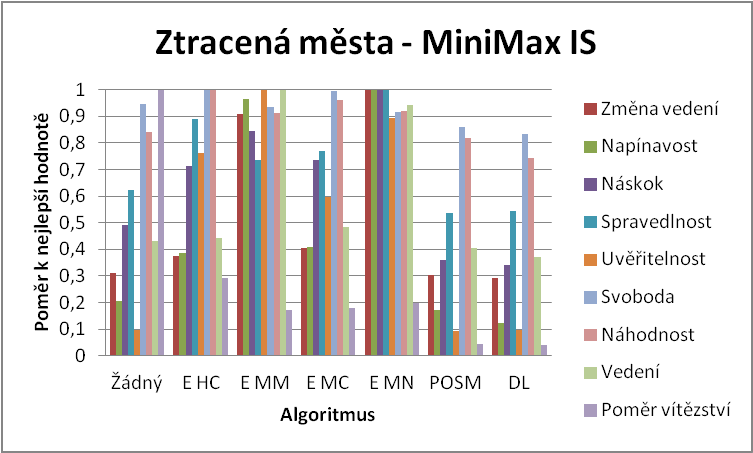
\includegraphics[width=0.75\textwidth]{ch5lcmm}
	\caption{Srovnání DDA alg. ve hře Ztracená Města s dvěma MiniMax IS hráči. (úrovně 50 a 100)}
	\label{fig-ch5lcmm}
\end{figure}

E-MC a E-HC dopadly navzájem podobně, ale oba lépe než hra bez DDA. Jelikož E-HC je znatelně rychlejší, je v tomto případě vhodnější než E-MC. Vítězem u Ztracených měst je jednoznačně E-MN, který byl nejlepší v metrikách změna vedení, napínavost, náskok a spravedlnost.

\section{Celkové srovnání}

Pro celkové srovnání použitých DDA algoritmů jsem každý algoritmus ohodnotil v jednotlivých hrách na základě všech 9 metrik a zvlášť na základě pouze 4 metrik změna vedení, napětí, náskok a poměr vítězství. Dvojí hodnocení jsem použil ze dvou důvodů. Algoritmy POSM a DL nebyly navrženy pro testování na daných metrikách a za druhé jejich použití u her Ludo a Ztracená města neovlivňuje 4 ze zbylých metrik.

Hodnocení algoritmu ve hře se rovná součtu hodnocení za jednotlivé metriky. Algoritmus, který si vedl nejlépe v daném metrice, získal celý bod za tuto metriku. Ostatní algoritmy si přičetly poměr jejich hodnoty k nejlepší hodnotě. Z toho vyplývá, že u prvního hodnocení je maximální hodnota 9, u druhého 4.

\begin{figure}
  \centering
  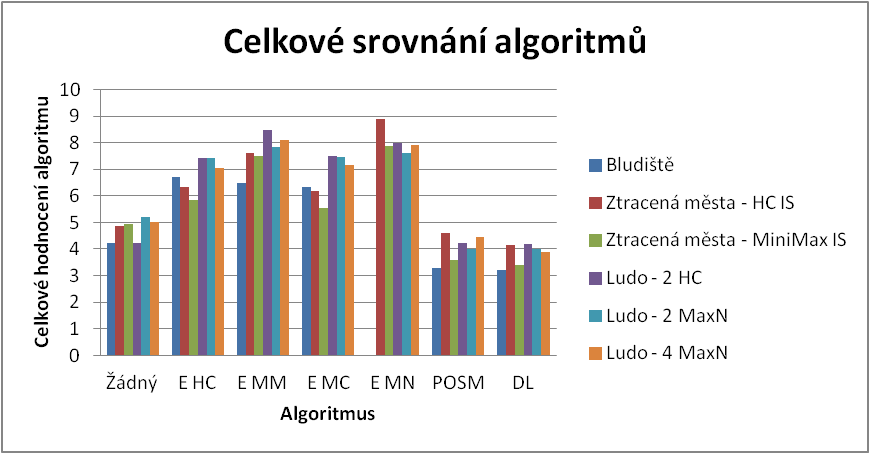
\includegraphics[width=0.80\textwidth]{ch5all}
	\caption{ Srovnání alg. DDA na základě všech experimentů a metrik. }
	\label{fig-ch5all}
\end{figure}

První hodnocení je znázorněno na grafu \ref{fig-ch5all} a v tabulce \ref{tab-all8m}. Nejlépe dopadly algoritmy E-MM a E-MN. E-MN získal ve Ztracených městech téměř maximální počet 9 bodů, získal 8,87. Za nimi následuje dvojice E-HC a E-MC se zisky kolem 6,5 bodů. DL s POSM dopadly nejhůře se zisky kolem 4 bodů.

\begin{table*}[b]\footnotesize
\vspace*{0mm}
\caption{{\label{tab-all8m}} Celkové hodnocení algoritmů v 6 experimentech na základě 9 metrik.}
\vspace*{0mm}
\label{shadowtable}
\begin{center}
\begin{tabular}{| l || r | r | r | r | r | r | r | r | r |}
\hline
Algoritmus & Bludiště & ZM-HC IS & ZM-MM IS & Ludo-2HC & Ludo-2MN & Ludo-4MN \\
\hline
\hline
Žádný & 4,21 & 4,88 & 4,94 & 4,23 & 5,22 & 5,03\\ \hline  
E-HC & 6,71 & 6,35 & 5,86 & 7,40 & 7,43 & 7,06\\ \hline  
E-MM & 6,47 & 7,62 & 7,48 & 8,47 & 7,85 & 8,10\\ \hline  
E-MC & 6,34 & 6,20 & 5,53 & 7,50 & 7,46 & 7,18\\ \hline  
E-MN & Neměřeno & 8,87 & 7,87 & 8,00 & 7,61 & 7,89\\ \hline  
POSM & 3,30 & 4,59 & 3,59 & 4,23 & 4,00 & 4,43\\ \hline  
DL & 3,23 & 4,14 & 3,38 & 4,20 & 3,99 & 3,87\\ \hline  
\end{tabular}
\end{center}
\end{table*}

Zaměříme-li se pouze na 4 zmíněné metriky, dojde ke stejným závěrům. Zajímavostí je, že ve hře Ztracená města s dvěma HillClimber hráči algoritmus E-MN dominoval ve všech 4 metrikách. DL a POSM i zde sbírají poslední místa.

Oba tyto algoritmy byly navrženy a testovány u her, kde jeden špatný tah zpravidla nerozhodne hru - testovanými hrami byl backgammon u DL a dáma s čínskými šachy u POSM.

\begin{figure}
  \centering
  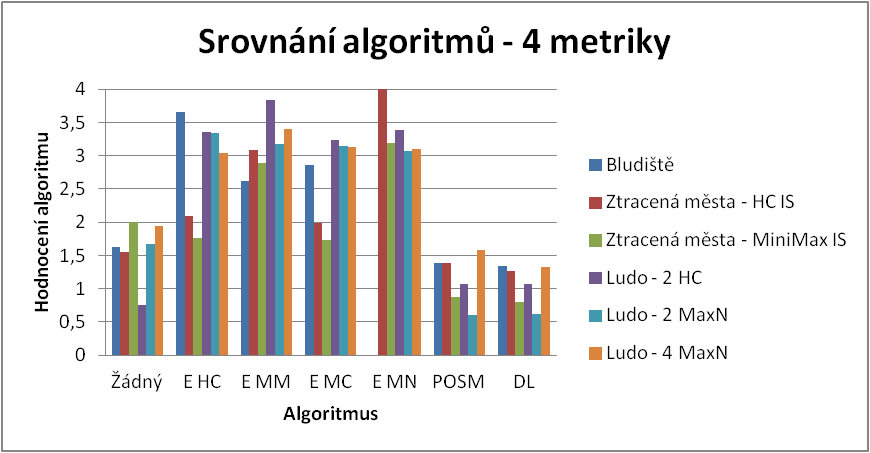
\includegraphics[width=0.80\textwidth]{ch5all4m}
	\caption{ Srovnání alg. DDA na základě všech experimentů a metrik Změna vedení, Napětí, Náskok a Poměr vítězů. }
	\label{fig-ch5all4m}
\end{figure}

Vzhledem výsledkům lze říci, že v případě dostatku výpočetního času a znalosti možných tahů hráčů, je nejvhodnější využít jeden z algoritmů E-MaxMax, nebo E-Max$^n$. Algoritmus založený na Monte Carlo prohledávání stromu dopadá obdobně jako E-HillClimber, ale má mnohem větší časovou náročnost a též potřebuje znalost možných tahů, a tedy se neukázal jako doporučitelný. E-HillClimber sice zaostává za první zmíněnou dvojicí, ale ne o moc. Průměrně dosáhl výsledku 6,8 bodů, E-MaxMax 7,7 a E-Max$^n$ 8,1. Z důvodu jednoduché implementace algoritmu a dobrým výsledkům může být E-HillClimber velice vhodným kandidátem na požití pro techniky DDA ve velikém spektru aplikací. Algoritmy dynamická úroveň a POSM se neukázaly být vhodné pro použití u tohoto typu her.

Pro doplnění E-MonteCarlo dosáhlo průměrně 6,7 bodů, POSM 4,0 a DL 3,8. Bez DDA se dosáhlo 4,8 bodů.

\begin{table*}[b]\footnotesize
\vspace*{0mm}
\caption{{\label{tab-all4m}} Celkové hodnocení algoritmů v 6 experimentech na základě 4 metrik - změna vedení, napínavost, náskok a poměr vítězství.}
\vspace*{0mm}
\label{shadowtable}
\begin{center}
\begin{tabular}{| l || r | r | r | r | r | r | r | r | r |}
\hline
Algoritmus & Bludiště & ZM-HC IS & ZM-MM IS & Ludo-2HC & Ludo-2MN & Ludo-4MN \\
\hline
\hline
Žádný & 1,62 & 1,54 & 2,01 & 0,76 & 1,67 & 1,94\\ \hline  
E-HC & 3,66 & 2,09 & 1,76 & 3,36 & 3,34 & 3,05\\ \hline  
E-MM & 2,62 & 3,09 & 2,89 & 3,83 & 3,18 & 3,39\\ \hline  
E-MC & 2,86 & 1,99 & 1,73 & 3,24 & 3,15 & 3,13\\ \hline  
E-MN & Neměřeno & 4,00 & 3,20 & 3,38 & 3,07 & 3,10\\ \hline  
POSM & 1,38 & 1,39 & 0,88 & 1,07 & 0,60 & 1,59\\ \hline  
DL & 1,34 & 1,27 & 0,79 & 1,08 & 0,62 & 1,33 \\ \hline  
\end{tabular}
\end{center}
\end{table*}

\endinput
%%
%% End of file `ch01.tex'.

	\chapter{Závěr}

Cílem diplomové práce bylo seznámit se s problematikou dynamického vyvažování obtížnosti v počítačových hrách především z hlediska algoritmů teorie her, zanalyzovat existující přístupy a metriky pro měření úspěšnosti jednotlivých přístupů, navrhnout nový přístup a metriky. Dalším cílem bylo navrhnout a implementovat testovací prostředí s třemi hrami a na nich nový přístup ohodnotit dle existujících i nových metrik. 

Nalezené existující přístupy využívají velké množství metod umělé inteligence. Jsou zde zastoupeny neuronové sítě, POMDP, fuzzy logika, evoluční algoritmy a další. DDA v oblasti teorie her se ukázalo být zatím nedostatečně prozkoumáno, a proto by tato práce měla částečně zaplnit tuto mezeru.

Navrhl jsem algoritmy založené na hráči prostředí, který má za úkol přizpůsobovat náhodné události a skrytou informaci. Při používání DDA je jedním z hlavních rizik hráčovo zjištění, že je DDA ve hře použito. Z tohoto důvodu bylo zásadní navrhnout algoritmy tak, aby upravovaly náhodné události v uvěřitelné míře. Pro tento účel se ukázala čtveřice existujících metrik zábavnosti - poměr vítězství, změna vedení, náskok a napětí - nedostatečná. Z tohoto důvodu jsem postupně dodefinoval další pětici metrik - doba vedení, uvěřitelnost, spravedlnost, svoboda a náhodnost, které existující metriky vhodně doplnily. Algoritmy založené na hráči prostředí jsem nazval E-HillClimber, E-MaxMax, E-MaxN a E-MonteCarlo dle známých algoritmů z teorie her, z kterých vycházejí.

Pro ověření funkčnosti nových algoritmů jsem navrhl a implementoval testující prostředí s třemi hrami - Bludiště, Ludo a Ztracená města. Aplikace obsahuje režim pro hraní hry člověkem proti soupeřům a režim dávkového spouštění experimentů na více vláknech.

Každý z experimentů jsem nejdříve spustil bez jakéhokoli mechanismu DDA, poté se čtveřicí algoritmů hráče prostředí a nakonec s dvěma existujícími algoritmy dynamická úroveň a POSM pro porovnání. Výsledky experimentů jsou pozitivní. Hráč prostředí se ukázal jako vhodným konceptem, který předčil hru bez žádného DDA mechanismu i algoritmy dynamickou úroveň a POSM ve všech třech testovaných hrách. 

V experimentech nejlépe dopadl E-MaxN, který v některých případech dokázal předčit všechny ostatní algoritmy dle většiny metrik. E-HillClimber dosáhl o něco slabších výsledků, ale stále oproti existujícím přístupům i proti nevyužití žádného DDA si vedl velmi dobře. E-HillClimber je jednoduchým algoritmem, který je díky svým malým požadavkům a velké rychlosti použitelný nejen v tahových hrách.

Do budoucna lze navázat na výstup této diplomové práce především otestováním algoritmů na lidech, důkladným zkoumáním vlivu změn koeficientů metrik u jednotlivých her, případně s návrhem jiné maximalizační funkce než je vážená suma metrik.

Diplomovou práci v této podobě považuji za kompletní. Věřím, že plně splnila zadání.

\endinput
%%
%% End of file `ch01.tex'.

  %...

  \startAppendices
    \chapter{Ovládání aplikace}

\section{Aplikace}

Aplikace byla naprogramována v jazyce C++ a používá knihovnu funkcí Qt. Na CD je přiložen projekt pro Visual Studio 2010 se všemi zdrojovými kódy. Dále je k dispozici zkompilovaná verze programu s potřebnými dynamickými knihovnami.

Pro spuštění zkompilované verze je potřeba pouze počítač s operačním systémem Windows. Aplikace se neinstaluje, stačí spuštění .exe souboru.

Ovládání aplikace by mělo být intuitivní. V hlavním menu jsou volby Nová hra, Změnit hru, Nastavení a Dávkové spouštění. Nová hra restartuje hru s novým nastavením. Ve změnit hru lze vybrat jednu ze tří implementovaných her a v Nastavení ji nakonfigurovat.

Menu Dávkové spouštění slouží k provádění experimentů. Zpět z Dávkového spouštění se uživatel dostane vybráním Nová hra z hlavní nabídky.


\begin{figure}
  \centering
  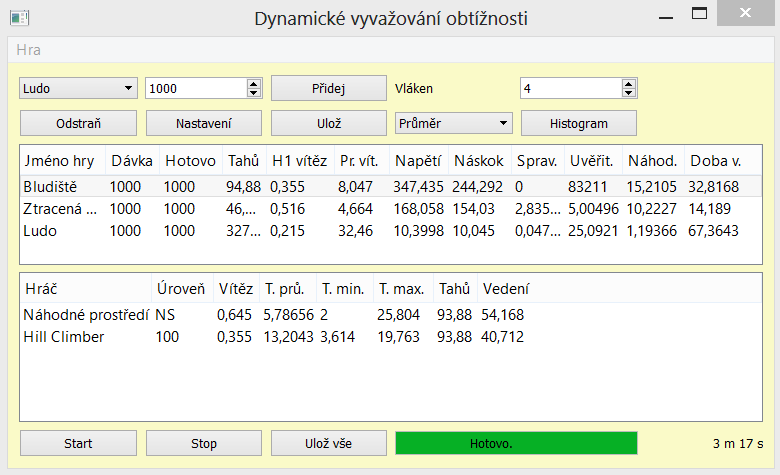
\includegraphics[width=0.90\textwidth]{appdavka}
	\caption{Uživatelské rozhraní dávkového spouštění experimentů. }
	\label{fig-appdavka}
\end{figure}

Uživatel přidá novou dávku zvolením dvou parametrů. Z výběrového menu vybere hru a nastaví počet iterací experimentu. Tlačítkem Přidej vytvoří jeden nový experiment, který se objeví v seznamu navolených experimentů. 

Po označení experimentu v seznamu může uživatel využívat čtveřici tlačítek Odstraň, Nastavení, Ulož, Histogram. Odstraň vymaže experiment z dávky, Nastavení otevře okno s nastavením pro hru, Ulož umožňuje uložit výsledky proběhlého experimentu, Histogram otevře okno, v kterém lze zobrazit jednotlivé metriky pro jeden experiment jako histogram. Dále je ve stejném řádku možnost voleb Průměr, Směrodatná odchylka, Minimum a Maximum. Dle volby se po proběhnutí experimentů v jejich seznamu zobrazují příslušné hodnoty z daných experimentů. 

\begin{figure}
  \centering
  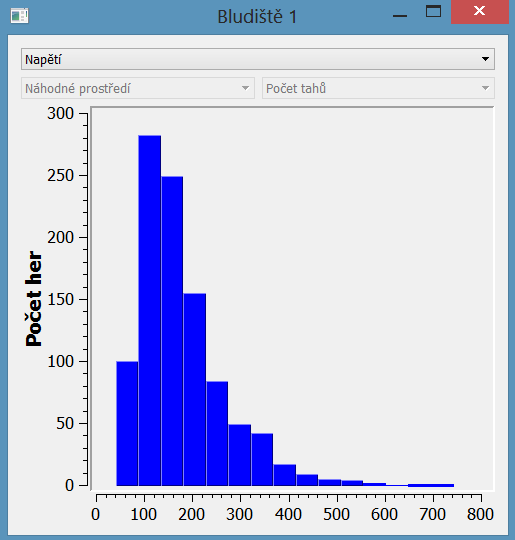
\includegraphics[width=0.75\textwidth]{apphistogram}
	\caption{Histogram metriky Napětí pro hru bludiště a 1000 iterací experimentu. }
	\label{fig-apphistogram}
\end{figure}

Pomocí tlačítka Start se spustí navolené experimenty jeden za druhým. Iterace v rámci jednoho experimentu se rozdělí do předem definovaného počtu vláken. Tlačítkem Stop se experimenty zastaví, ale nechají se doběhnout aktuálně rozehrané hry. Pomocí tlačítka Uložit vše lze hromadně uložit výsledky všech experimentů do zvolené složky. 

V průběhu experimentu se zobrazuje uplynulý čas a velice hrubý odhad skončení experimentů. Spočítá se dle průměrné doby na jednu iteraci od začátku spuštění experimentů a dle počtu zbylých iterací ve všech experimentech.

Po označení experimentu v seznamu se zároveň zobrazí ve spodním okně několik metrik k jednotlivým hráčům. Pro každého hráče je uvedeno jeho jméno, úroveň, poměr vítězství. T. prů. T. min., T. max. značí průměrný, minimální a maximální počet tahů hráče během hry. Poslední dvě metriky znamenají kolikrát byl hráč na tahu a kolik kol byl ve vedení.

V seznamu experimentů se zobrazuje jméno hry, celkový a proběhlý počet iterací experimentu, celkový počet tahů, poměr vítězství prvního hráče a metriky prohození vítězů, napětí, náskok, spravedlnost, uvěřitelnost, náhodnost, doba vedení v tomto pořadí.

\section{Hry}

V této části stručně popíši uživatelské rozhraní jednotlivých her. Nezmiňuji zde pravidla her, která byla uvedena v páté kapitole.

Nastavení her je stejné pro dávkové spouštění i při hraní člověk proti počítači. V levé polovině uživatel může nastavit algoritmy pro jednotlivé hráče a případně jejich úroveň, pokud to daný algoritmus umožňuje. Pod nastavením hráčů jsou speciální nastavení pro jednotlivé hry popsány níže.

V pravé části nastavení se volí hráč prostředí a koeficienty pro jednotlivé metriky. Nastavení se stane platné až po uložení tlačítkem Uložit a po spuštění nové hry.

\subsection{Bludiště}

Hra se ovládá pomocí levého tlačítka myši. Hráč ovládá žlutou kuličku a snaží se dostat včas ke všem bombám, které jsou na mapě znázorněny zelenými čtverci. Hráč vždy kliknutím vybere, které další dveře se mají otevřít. K otevřeným dveřím postava dojde skokem. Dveře jsou znázorněny oranžovými, modrými a červenými čtverci. Dle barvy dveří a jejich vzdálenosti od předchozí pozice, se hráči odečtou zbývající kroky do konce hry.

\begin{figure}
  \centering
  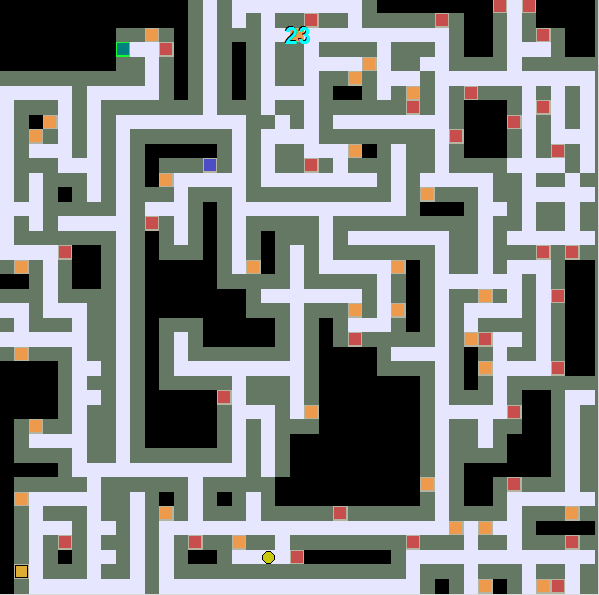
\includegraphics[width=0.75\textwidth]{appmaze}
	\caption{Uživatelské rozhraní hry Bludiště. Zelený čtverec představuje možnou bombu. }
	\label{fig-appmaze}
\end{figure}

Zbývající počet kroků do konce hry zobrazuje tyrkysové číslo v horní části hry. 

V případě, že některá bomba se stane nedostupnou, tak byla falešná a zmizí z mapy.

\emph{Speciální nastavení} : Před hrou hráč může upravit parametry velikosti bludiště a počáteční limit na počet kroků.

\subsection{Ludo}

Hra Ludo se také ovládá pomocí myši. Kostkou se hází automaticky. Hodnota, která padla, je znázorněna uprostřed herní plochy. Hráč může pohnout s figurami, které jsou na bíle zvýrazněném poli. Jestliže figurkou nemůže pohnout, tak buď mu v tom brání vlastní figurka, kterou by jinak vyhodil, nebo je před figurkou již obsazené bezpečné místo.

\begin{figure}
  \centering
  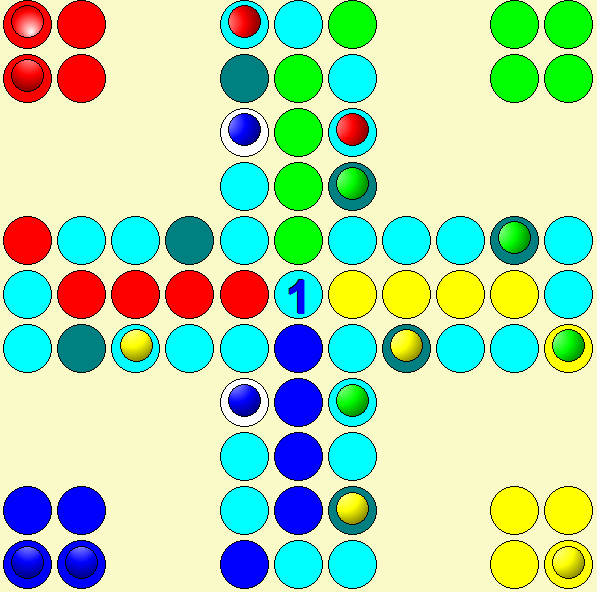
\includegraphics[width=0.75\textwidth]{appludo}
	\caption{Uživatelské rozhraní hry Ludo. Bílý podklad značí aktivní figurky. }
	\label{fig-appludo}
\end{figure}

Bezpečná místa jsou zvýrazněna tmavší barvou.

V případě, že hráč nemá ani jednu figurkou na hlavním plánu, hází kostkou až třikrát. Pouze první hod se provede automaticky, ostatní hody provádí hráč kliknutím doprostřed herního pole.

\emph{Speciální nastavení} : Lze nastavit hru pouze dvou hráčů. V takovém případě se ignoruje nastavení druhého a čtvrtého hráče.

\subsection{Ztracená města}

Hra se opět ovládá pouze pomocí levého tlačítka myši. Každý tah se vždy skládá ze třech kliknutí. Prvním kliknutím na kartu v ruce hráč vybere, s kterou kartou bude hrát. 

Při druhém kliknutí hráč vybírá, co s kartou udělá. Může jí buď zahodit vybráním příslušného odkládacího balíčku, které jsou na začátku hry znázorněny šedivým čtvercem se zaoblenými hranami. V případě, že kartu může zahrát, klikne pod odkládací balíček dané barvy. 


\begin{figure}
  \centering
  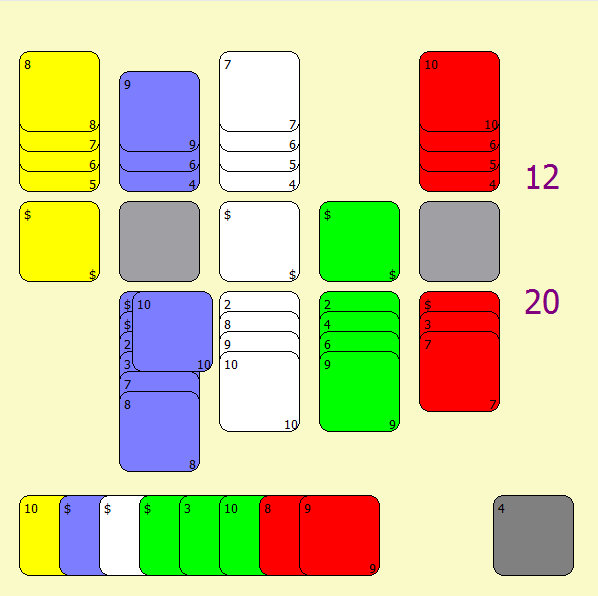
\includegraphics[width=0.75\textwidth]{applc}
	\caption{Uživatelské rozhraní hry Ztracená města. }
	\label{fig-applc}
\end{figure}

Nakonec třetím kliknutím hráč vybere, odkud dobere kartu. Jedna z možností je dobrat z dobíracího balíčku, který je znázorněn šedivě v pravém dolním rohu. Je na něm číslo udávající počet zbývajících karet v balíčku. V případě, že jsou na stole odložené karty, může hráč kliknout na jednu z nich a vzít si ji do ruky.

Uživateli se vždy zvýrazňují oblasti ve hře, které jsou zrovna aktivní a hráč na ně může kliknout.

\emph{Speciální nastavení} : Lze nastavit počet karet v ruce. Oficiální pravidla hry umožňují variantu 8 a 5 karet v ruce.

\endinput
%%
%% End of file `ch01.tex'.

		\chapter{Doplňující grafy experimentů}

\begin{figure}
  \centering
  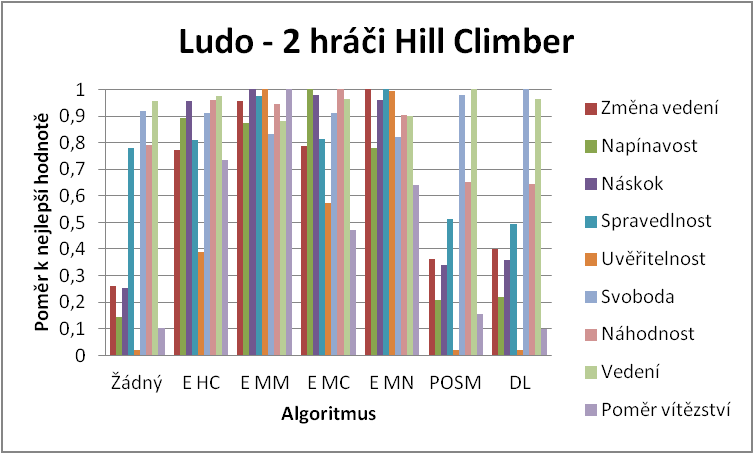
\includegraphics[width=0.75\textwidth]{ch5ludo2hc}
	\caption{Srovnání DDA alg. ve hře Ludo se dvěma Hill Climber hráči. (úrovně 50 a 100)}
	\label{fig-ch5ludo2hc}
\end{figure}

\begin{figure}
  \centering
  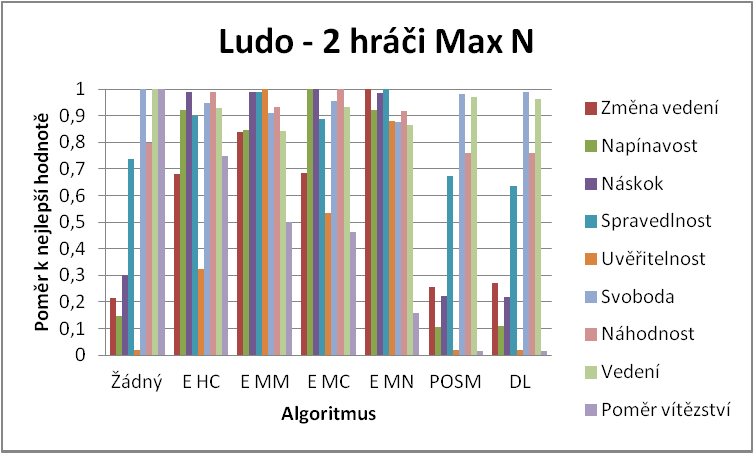
\includegraphics[width=0.75\textwidth]{ch5ludo2maxn}
	\caption{Srovnání DDA alg. ve hře Ludo se dvěma Max N hráči. (úrovně 50 a 100)}
	\label{fig-ch5ludo2maxn}
\end{figure}

\begin{figure}
  \centering
  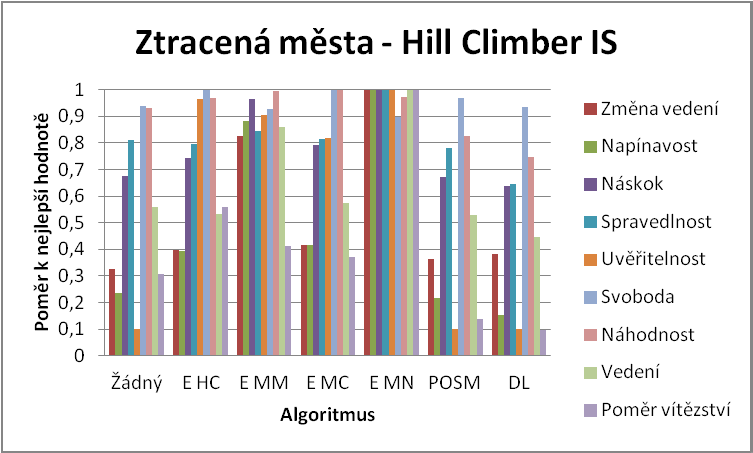
\includegraphics[width=0.75\textwidth]{ch5lchc}
	\caption{Srovnání DDA alg. ve hře Ztracená města se Hill Climber IS hráči. (úrovně 50 a 100) }
	\label{fig-ch5lchc}
\end{figure}


\endinput
%%
%% End of file `ch01.tex'.

  \stopAppendices
\stopBodyMatter

\startBackMatter
  \PrintBibliography
  %\PrintIndex % define index entry in the text by: \index{word}
\stopBackMatter

\end{document}

\endinput
%%
%% End of file `template.tex'.
